%&../.preamble
\endofdump

\usetikzlibrary{external}
\usetikzlibrary{patterns}
\usepackage[outline]{contour}
%\tikzset{external/system call={pdflatex -fmt=../.preamble.fmt \tikzexternalcheckshellescape -halt-on-error -interaction=batchmode -jobname "\image" "\texsource"}}
\tikzset{external/system call={pdflatex --shell-escape --fmt=../.preamble --halt-on-error -jobname "\image" "\endofdump\texsource"}}
\tikzexternalize[prefix=tikz/]

\title{Statistica}
\author{Mattia Marini}

\begin{document}
\maketitle
\tableofcontents
\section{Tribù e algebre}
E' spesso necessario sceglere i possibili eventi all'interno di una classe che presenti caratteristiche particolari, ossia una \underline{tribù}
\definizione{Tribù}{
	Data una classe $ \mathcal{A} $ su uno spazio campionario $ \omega  $ si dice \underline{tribù} se soddisfa le seguenti proprietà:
	\begin{enumerate}
		\item $ \omega \in \mathcal{A}$
		\item se $ A \in  \mathcal{A} $ allora $ A^{c} \in  \mathcal{A} $
		\item Se $ A_1, A_2,\ldots,A_i, \ldots \in \mathcal{A} $ allora $ \bigcup_{i=1}^{+ \infty }A_i \in \mathcal{A} $
	\end{enumerate}
}
\definizione{Algebra}{
	Data una classe $ \mathcal{A} $ su uno spazio campionario $ \omega  $ si dice \underline{tribù} se soddisfa le seguenti proprietà:
	\begin{enumerate}
		\item $ \omega \in \mathcal{A}$
		\item se $ A \in  \mathcal{A} $ allora $ A^{c} \in  \mathcal{A} $
		\item Se $ A_1, A_2,\ldots,A_i, \ldots \in \mathcal{A} $ allora $ \bigcup_{i=1}^n A_i \in \mathcal{A} $
	\end{enumerate}
}
In particolare nota che
\begin{itemize}
	\item \textit{Proprietà 2:} garantisce che se un evento $ E $ si può verificare, allora si può verificare anche $ E^{c} $
	\item  \textit{Proprietà 3:} garanisce che se si possono verificare gli eventi $ E_1,\ldots,E_i $ allora si può verificare anche l'evento $ E_1 \cup  E_2 \cup \ldots \cup  E_i $.
\end{itemize}
\teorema{Tribù e algeebra}{
	Un'\underline{algebra} è anche una \underline{tribù}, tuttavia \underline{non} vale il contrario
}
Dimostrzione:
\begin{itemize}
	\item Per definizione una tribù contine $ \omega  $ e di ogni elemento contiene anche il \underline{complementare}. Quindi ogni tribù contiene $ \emptyset  $.
	\item Data una tribù, l'unione di un numero finito di suoi elementi sta in questa. Ma anche l'unione di un numero infinito di suoi elementi, in quanto posso aggiungere \underline{infiniti insiemi vuoti}
\end{itemize}

\definizione{Evento}{
	Un elemento di una tribù $ \mathcal{A} $ si dice \underline{evento}.
}
\definizione{Spazio probabilizzabile}{
	Dato uno spazio campionario $ \omega  $ e una tribù $ \mathcal{A} $ la coppia
	\[
		\left(\omega , \mathcal{A}\right)
	\]
	è detta \underline{spazio probabilizzabile}
}

\definizione{Spazio probabilizzato}{
	Dato $ \omega  $ e una tribù $ A $ di $ \omega $ e una probabilità $ P $ sullo \underline{spazio probabilizzabile} (ossia la coppia $ \omega $, $ A $), chiameremo la terna
	\[
		(\omega, A, P)
	\]
	uno \underline{spazio probabilizzato}
}

\definizione{Probabilità (versione assiomatica Kolmogorov)}{
	Dato uno spazio proabilizzabile $ \left(\omega , \mathcal{A}\right) $ la \underline{probabilità} è un'applicazione $ Pr: \mathcal{A} \to \R ^{+} $  tale che:
	\begin{itemize}
		\item \textit{Non negatività:} Se $A \in \mathcal{A} $ allora $ Pr\left(A\right) \ge 0 $
		\item \textit{Normalizzazione:}$ \Pr\left(\omega \right)=1 $
		\item \textit{$ \sigma $ addittività:} Data una serie di eventi incompatibili, la probabilità dell'unione di questi è la somma delle probabilità di ogni evento, formalmente:
		      \[
			      \forall A_j, A_j \text{ t.c. } A_i \cap A_j = \emptyset i \neq j \quad \Rightarrow \quad Pr\left(\bigcup _{i=1}^{\infty }A_i\right) = \sum_{i=1}^{\infty} Pr\left(A_i\right)
		      \]
	\end{itemize}
}
\subsubsection*{Esempio 1}
Pendo un insieme e una tribù:
\[
	\omega = \left\{1,2,3,4,5,6\right\} \quad \mathcal{A} = P\left(\omega\right)
\]
\[
	\left(\omega , \mathcal{A} \right) \text{ è uno spazio probabilizzabile} \quad Pr\left(\left\{1\right\}\right)= Pr\left(\left\{2\right\}\right) = \ldots = Pr\left(\left\{6\right\}\right) = p
\]
Per procedere formalmente devo applicare gli assiomi:
\[
	Pr\left(\omega \right)= 1= Pr\left(\left\{1\right\} \cup  \left\{2\right\} \cup   \ldots \cup  \left\{6\right\} \right)= \sum_{k=1}^{6} Pr\left(\left\{i\right\}\right) = 6p
\]
il tutto è uguale a $ 6p $ visto che ho supposto che gli eventi elementari avessero la stessa probabilità. Quindi
\[
	p=\frac{1}{6}
\]
Se ora dovessi ricavare la probabilità di un insieme generico posso utilizzare $ p $ per farlo:
\[
	P\left(\left\{1,3,5\right\}\right) = P\left(\left\{1\right\},\left\{3\right\},\left\{5\right\}\right)=P\left(\left\{1\right\}\right)+ P\left(\left\{3\right\}\right) + P\left(\left\{5\right\}\right)=\frac{3}{6} = \frac{1}{2}
\]
\subsubsection*{Esempio 2}
Immagino di prendere un bersaglio di raggio $ r $ e di voler calcolare la probabilità di colpire ognuna delle parti. Assumo che non sia possibile colpire fuori dal pannello e che la probabilità di colpire ciascuna porzione sia direttamente proporzionale alla sua area.
\begin{align*}
	P\left(\left\{3\right\}\right) & = \frac{\pi \left(\frac{1}{3}r\right)^2}{\pi r^2} = \frac{1}{9}                                   \\
	P\left(\left\{2\right\}\right) & = \frac{\pi \left(\frac{2}{3}r\right)^2 - \pi \left(\frac{1}{3}r\right)^2}{\pi r^2} = \frac{1}{3} \\
	P\left(\left\{1\right\}\right) & = \frac{\pi r^2 - \pi \left(\frac{2}{3} r\right)^2 }{\pi r^2 } = \frac{5}{9}
\end{align*}
\subsection{Regole importanti}
\begin{itemize}
	\item  \textbf{Regola 1} $ \left(\omega , \mathcal{A}, P\right) $ Allora $ Pr\left(A^{c}\right) = 1-Pr\left(A\right) $
	\item \textbf{Regola 2} $ \left(\omega , \mathcal{A}, P\right) $ se $ A, B \in A $ allora $ P\left(A \cup B\right) = P\left(A\right) + P\left(B\right) - P\left(A \cap B\right) $
	      \begin{itemize}
		      \item Se $ A, B $ sono disgiunti, allora posso applicare l'assioma di unione di insiemi disgiunti e sono a posto
		      \item Se $ A,B $ \underline{NON} sono disgiunti, allora applico il seguente trucco:
		            \[
			            A \cup B = A \cup\left(B \cap A^{c}\right)
		            \]
		      \item Gli insiemi $ A $ e $ \left(A \cap A^{c}\right) $ sono disgiunti e posso dunque applicare l'assioma
	      \end{itemize}
	\item \textbf{Regola 3} Se $ A \subset B $ allora $ P\left(A\right) \le P\left(B\right) $
	      \begin{itemize}
		      \item $ B = \left(A \cap B\right) \cup \left(A^{c}\cap B\right) $
		      \item Siccome $ A \subset B $ allora $ B= A \cup\left(A^{c}\cap B\right) $
	      \end{itemize}
	\item \textbf{Regola 4} \textit{(Disuguaglianza di Bonferroni)}. Se $A_1, A_2, \cdots, A_n$ sono eventi allora
	      \[
		      \sum_{i=1}^n \Pr\left(A_i\right)-\sum_{1 \leq i \leq j \leq n} \Pr\left(A_i \cap A_j\right) \leq \Pr\left(\cup_{i=1}^n A_i\right) \leq \sum_{i=1}^n \Pr\left(A_i\right), \quad n \geq 1
	      \]
\end{itemize}
\definizione{}{
Data una famiglia di spazi probabilizzabili $ \left\{\left(\omega _i, A_i\right)\right\}_{i \in  I} $, possiamo costruire uno spazio probabilizzabile prodotto ottenuto come pr odotto cartesiano
}
\definizione{Disposizioni con ripetizioni}{
	Sia $ S = \left\{a_1,a_2,\ldots , a_n\right\} \quad \#s = n $ un insieme costituito da oggetti distinti. Il numero di \underline{allineamenti} che si possono formare con \underline{r} oggetti scelti tra gli $ n $ si indica con $ D_{n,r}^{*} $. Due allineamenti sono diversi se una delle seguenti condizioni è verificata:
	\begin{itemize}
		\item Contengono \underline{oggetti divisersi}
		\item Contengono stessi oggetti in \underline{numero diverso}
		\item lo stesso oggetto si ripete un \underline{numero diverso di volte}
	\end{itemize}
	\[
		D_{n, r}^{*} = n ^{r}
	\]
}
\section{Calcolo combinatorio}
\definizione{Disposizione senza ripetizione}{
	Sia $ S = \left\{a_1,a_2,\ldots , a_n\right\} \quad \#s = n $ un insieme costituito da oggetti distinti. Il numero di \underline{allineamenti} che si possono formare con \underline{r} oggetti scelti tra gli $ n $ si indica con $ D_{n,r} $. Due allineamenti sono diversi se una delle seguenti condizioni è verificata:
	\begin{itemize}
		\item Contengono \underline{oggetti divisersi}
		\item Contengono stessi oggetti in \underline{numero diverso}
	\end{itemize}
	\[
		D_{n,r} = n \cdot  \left(n-1\right) \cdot  \ldots \cdot \left(n-r +1\right)=\frac{n!}{\left(n-r\right)!}
	\]
}
\definizione{Permutazioni}{
	Le permutazioni di $ n $ oggetti non sono altro che le \underline{disposizioni senza ripetizione} di $ n  $ oggetti in $ n $ posizioni:
	\[
		P_n = D_{n,n} = n!
	\]
}
\definizione{Combinazioni}{
	Sono date da tutti gli isiemi contenenti \underline{oggetti diversi} (ossia non conta l'ordine con il quale questi vengono disposti).
	\[
		C_{n,r} = \frac{D_{n,r}}{P_r} = \frac{n!}{\left(n-r\right)! \cdot r!} = \binom{n}{r}
	\]
	Ossia quanti gruppi di $ r $ persone posso estrarne da $ n $
}
\subsection{Esercizi}
\subsubsection*{Esercizio 1}
Immaginiamo di avere un comitato di 5 persone su 10.
\begin{itemize}
	\item Una persona può comparire nel comitato al più una volta
	\item L'ordine con il quale le persone appaiono i nomi nel comitato \underline{non} è importante
\end{itemize}
Ciò significa che devo utilizzare le \underline{combinazioni}:
\[
	C_{10, 5} = \frac{10!}{5!\cdot 5!} = \frac{10 \cdot  9 \cdot  8 \cdot  7 \cdot  6}{5!} = 252
\]
\subsubsection*{Esercizio 2}
Supponiamo di avere $ \omega_i = \left\{1,\ldots , 100\right\} \quad i = 1,2,3  $
\[
	\omega  = \bigtimes_{i=1}^{3} \omega_i
\]
supponendo di avere $ 6 $ volcali, il numero di parole che abbiano una consonante come primo , mentre una vocale come secondo e terzo è:
\[
	\frac{20 \cdot  6 \cdot  6 }{100 ^{3} } = 0,00072
\]
\subsubsection*{Esercizio 3}
Supponiamo di avere un insieme così definito:
\[
	\left\{A_1, A_2,A_2,A_4,A_5,B_1,B_2,C_1,D_1,R_1,R_2\right\}
\]
immagina di estrarre da un vaso una lettera alla volta, senza riimmetterla dopo ogni estrazione. Calcola la probabilità di aver estratto le lettere in questo ordine:
\[
	\left\{A,B,R,A,C,A,D,A,B,R,A\right\}
\]
innanzitutto, $ \omega = P_11 = 11! $. Inoltre mi immagino che ogni lettera ripetuta può essere permutata (in quanto non cambierebbe avere $ A_1 $ o $ A_2 $ in posizione 1). Dunque prendendo la stringa \textit{ABRACADABRA} devo considerare ogni possibile ordine delle a, delle b e così via:
\[
	P\left("ABRACADABRA"\right) = \frac{5! \cdot  2! \cdot 1! \cdot 1! \cdot 2!}{11!} = \frac{1}{83160}
\]
\subsubsection*{Esercizio 4}
Viene somministrato un trattamento (T) e un placebo (C) a maschi e femmine
\begin{table}[h!]
	\centering
	\begin{tabular}{|c c c c|}
		\hline
		T & M & S & 8  \\
		C & M & S & 4  \\
		T & F & S & 12 \\
		C & F & S & 2  \\
		\hline
	\end{tabular}
	\begin{tabular}{|c c c c|}
		\hline
		T & M & I & 5  \\
		C & M & I & 3  \\
		T & F & I & 15 \\
		C & F & I & 3  \\
		\hline
	\end{tabular}
\end{table}
Nota che la differenza di efficacia fra placebo e trattamento dipende dal sesso in quanto:
\begin{align*}
	P\left(S | T\right) & = \frac{8 + 12}{8 + 12 + 5 + 15} = \frac{1}{2} \\
	P\left(S | c\right) & = \frac{4 + 12}{4 + 2 + 3 + 3} = \frac{1}{2}
\end{align*}
tuttavia, nota che:
\begin{align*}
	P\left(S | T, M\right)  & = \frac{ 8}{ 8 + 5}= \frac{8}{13}    \\
	P\left(S | C , M\right) & = \frac{4}{4 + 3} = \frac{4}{7}      \\
	P\left(S | T , F\right) & = \frac{12}{12 + 15} = \frac{12}{27}
\end{align*}
\subsection{Teorema di Bayes}
\teorema{Teorema di Bayes}{
Abbiamo una successione di eventi $ \left\{ A_i\right\}_{i = 1}^{+ \infty } $ che formi una partizione di $ \omega  $. Assumiamo che $ P\left(A_i\right)> 0 \forall  i $. Prendo un $ b \in \mathcal{A} \text{ t.c. } P\left(B\right)> 0 $
\[
	P\left(A_i | B\right) = \frac{P\left(B|A_i\right)\cdot P\left(A_i\right)}{\sum_{j=1}^{\infty} P\left(B|A_j\right)\cdot  P \left(A_j\right)}
\]
}
\definizione{Indipendenza stocastica}{
	Dato $ \left(\omega, \mathcal{A}, P\right) $ e due eventi $ A, B $ diremo che sono tra loro \underline{stocasticamente indipendenti} se e solo se:
	\[
		P\left(A \cap B\right)= P\left(A \right) \cdot P\left(B\right)
	\]
}
Ciò significa che i due eventi \underline{non} si influenzano a vicenda:
\[
	P\left(A|B\right)= \frac{P\left(A \cap  B\right)}{P(B)\left(B\right)} = \frac{P (A) \cdot P\left(B\right) }{P\left(B\right)} = P\left(A\right)
\]
\section{Probabilità sui reali}
Costruiamo uno spazio probabilizzato che veda come spazio campionario $ \R  $:
\begin{itemize}
	\item Per questioni di semplicità, noi considereremo $ \Omega = \R $
	\item Dobbiamo ora definire una \textit{tribù}. La tribù $ \mathcal{P}\left(\R \right) $ tuttavia contiene degli insiemi che non sono di nostro interesse (vedi \textit{insiemi di vitali})
\end{itemize}
\subsection{Insiemi di Bourelliani}
L'idea di base è quela di considerare solo insiemi per i quali ha senso parlare della loro \textit{lunghezza} (o area e volume rispettivamente in $ \R ^{2} $ e $ \R ^{3} $)
Per costruire questo insieme procediamo così:
\begin{itemize}
	\item Prendiamo l'insieme dato da ogni sottointervallo del tipo $ (a,b] $ di $ \R  $ così definito:
	      \[
		      \mathcal{F}=\{(a, b]: a \leq b ; a, b \in \mathbb{R}\}
	      \]
	\item Dobbiamo ora creare una tribù a partire da questo insieme. In particolare prendiamo la più piccola tribù che contiene ogni sotto intervallo di $ \R  $:
	      \[
		      \mathcal{A}_{\mathcal{F}} = \cap \left\{\mathcal{A}: \mathcal{A}: \text{ è una tribù e } \mathcal{F} \subseteq \mathcal{A} \right\}
	      \]
\end{itemize}
La tribù $ \mathcal{A}_{\mathcal{F}} $ è detta \underline{tribù dei Boreliani}. La tribù contiene i seguenti elementi:
\begin{itemize}
	\item $(a, b)$
	\item $[a, b]$
	\item $[a, b)$
	\item $(-\infty, b]$
	\item $(a, \infty)$
	\item i singoletti di $\mathbb{R}$;
	\item gli insiemi finiti di $\mathbb{R}$;
	\item gli insiemi numerabili di $\mathbb{R}$.
\end{itemize}
\textbf{Dimostrazione:}
Partiamo dimostrando che $ \left(a,b\right) \in \mathcal{A}_{\mathcal{F}} $.
\begin{itemize}
	\item $ \left(a,b\right) $. Definiamo la seguente successione:
	      \[
		      \bigcup_{k = 1}^{\infty } \left(a, b - \frac{1}{k}\right]
	      \]
	      Chiaramente per $ k \to  \infty  $ la successione tende a $ \left(a,b\right) $. Visto che l'unione numerabile di elementi di una tribù sta nella tribù stessa, $ \left(a,b\right) \subset \mathcal{A}_{\mathcal{F}} $
	\item $ \left(-\infty , b\right] $. Per lo stesso motivo di prima, $ \bigcup _{k=1}^{-\infty } \left(k, b\right] \to \left(-\infty , b\right) $
	\item $ \left(a, \infty \right) $. Visto che $ \left(-\infty, b \right] \in \mathcal{A}_{\mathcal{F}}$ allora anche il suo negato appartiane
	\item $ \left[a,b\right] $. Considero l'insieme seguente: $ \left(-\infty, b\right] \cup \left(b, c\right) \cup \left(d, \infty \right) $:
	      \vskip3mm
	      \begin{center}
		      \begin{tikzpicture}
			      \draw (0,0)--(4,0);
			      \draw [red!45](2,0)--(3,0);
			      \draw [dashed](-0.5,0)--(0,0);
			      \draw [dashed](4,0)--(4.5,0);
			      \draw [dotted](0,0)|-(2,-0.5)--(2,0);
			      \draw [dotted](3,0)|-(4,-0.5)--(4,0);
			      \draw [dotted](1,-0.5)--++(0,-0.5)--++(2.5, 0)node[pos = 0.5, anchor = north] {$ \left(-\infty, b\right] \cup \left(b, c\right) \cup \left(d, \infty \right) $}-++(0,0.5);
			      \node [anchor = north] {$  $};
			      \node [label=90:$ -\infty $] at (0,0){};
			      \node [label=90:$ \infty $] at (4,0){};
			      \node [blackdot, label=90:$ b $] at (1,0){};
			      \node [whitedot, label=90:$ c $] at (2,0){};
			      \node [whitedot, label=90:$ d $] at (3,0){};
		      \end{tikzpicture}
	      \end{center}
	      negando questo intervallo otteniamo chiaramente $ \left[a,b\right] $
	\item $ \left[a,b\right) $. Considero l'insieme seguente: $ \left(-\infty, b\right] \cup \left(b, c\right) \cup \left[d, e \right] \cup \left(e, \infty \right) $:
	      \vskip3mm
	      \begin{center}
		      \begin{tikzpicture}
			      \draw (0,0)--(5,0);
			      \draw [red!45](2,0)--(3,0);
			      \draw [dashed](-0.5,0)--(0,0);
			      \draw [dashed](5,0)--(5.5,0);
			      \draw [dotted](0,0)|-(2,-0.5)--(2,0);
			      \draw [dotted](3,0)|-(5,-0.5)--(5,0);
			      \draw [dotted](1,-0.5)--++(0,-0.5)--++(2.5, 0)node[pos = 0.5, anchor = north] {$ \left(-\infty, b\right] \cup \left(b, c\right) \cup \left[d, e \right] \cup \left(e, \infty \right)$}-++(0,0.5);
			      \node [anchor = north] {$  $};
			      \node [label=90:$ -\infty $] at (0,0){};
			      \node [label=90:$ \infty $] at (5,0){};
			      \node [blackdot, label=90:$ b $] at (1,0){};
			      \node [whitedot, label=90:$ c $] at (2,0){};
			      \node [blackdot, label=90:$ d $] at (3,0){};
			      \node [blackdot, label=90:$ e $] at (4,0){};
		      \end{tikzpicture}
	      \end{center}
\end{itemize}


Dato uno spazio campionario e una tribù (dei \textit{bourelliani}), manca solo definire la funzione di probabilità. Tale funzione è detta funzione di distribuizione:
\definizione{Funzione di distribuzione o ripartizione}{
	Una \underline{funzione di distribuzione} si $  \left(\R , B\left(\R \right)\right) $ $ F\left(x\right) $ è una funzione di distribuzione se:
	\begin{itemize}
		\item Non decrescente: $ x_1 < x_2 \Rightarrow  F\left(x_1\right) \le F\left(x_2\right) $
		\item Continua a destra: $ \lim_{x \to x_0^{+}} F\left(x\right) = F\left(x_0\right) $
		\item $ \lim_{x \to -\infty } F\left(x\right) = 0 $ e $ \lim_{x \to +\infty } F\left(x\right)=1 $
	\end{itemize}
	Data una funzione che rispecchi queste proprietà, la probabilità di un intervallo $ P\left((a,b]\right) $ è data da:
	\[
		F\left(b\right) - F\left(a\right)
	\]
	mentre la probabilità del singoletto $ P\left(\left\{x\right\}\right) $ è data da:
	\[
		F\left(x\right) - \lim_{z \to x^{-}} F\left(z\right)
	\]
}

\subsection{Esempi}
Consideriamo il seguente esperimento: \textit{calcola la probabilità di estrarre un punto nell'intervallo $ \left[0,1\right] $ nei numeri reali $ \R $}. Avremo dunque
\[
	\omega = \left[0,1\right] \in \R \quad \mathcal{A}_{\mathcal{F}} = \mathcal{B}\left[0,1\right] \quad P\left(\left(a,b\right]\right) = a-b
\]
Quindi la probabilità di estrarre un punto appartenente ad un intervallo $ \left(a,b\right] $ corrisponde alla sua lunghezza. La funzione di probabilità sarà la seguente:
	\begin{center}
			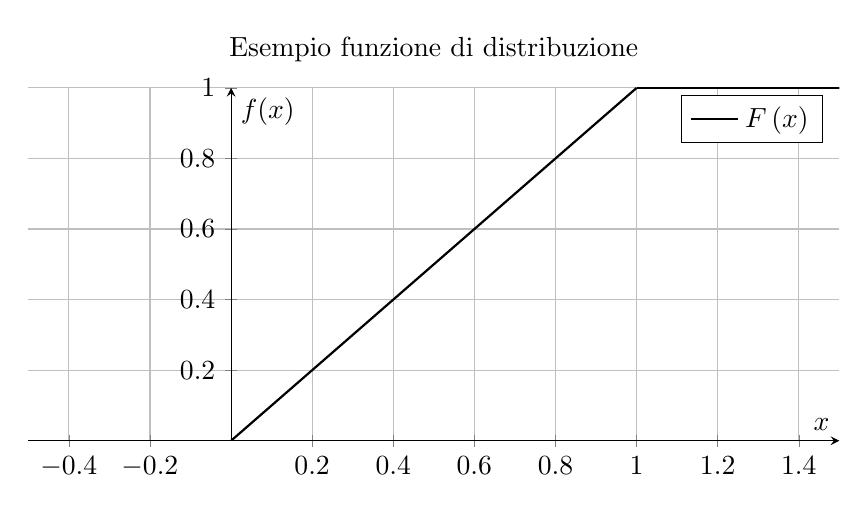
\begin{tikzpicture}
				\begin{axis}[ title = Esempio funzione di distribuzione,
						axis lines = center,
						xmin=-0.5, xmax=1.5,
						ymin=0,ymax=1,
						restrict y to domain = -1:3, domain=0:1, width=0.98\textwidth, height=0.5\textwidth, grid=major, samples=200,  ylabel=$f(x)$, xlabel=$x$, legend entries={$F\left(x\right)$}]
					\addplot[black, thick] {x};
					\addplot[black, thick, domain = -15:0] {0};
					\addplot[black, thick, domain = 1:15] {1};
				\end{axis}
			\end{tikzpicture}
			Calcoliamo ora le probabilità dei seguenti eventi.
			\begin{itemize}
				\item $A_1=\left\{\left(0, \frac{1}{4}\right)\right\}$
				\item $A_2=\{a\}$
				\item $A_3=\left\{a_1, a_2, \cdots\right\}$
				\item $A_4=\left\{\left[\frac{1}{2}, \frac{3}{4}\right] \cup\left[\frac{4}{5}, 1\right]\right\}$
				\item $A_5=[0,1] / A_3$;
				\item $A_6=\cup_{n=1}^{\infty}\left[\frac{k}{k+1}, \frac{k}{k+1}+\frac{1}{10^k}\right]$
			\end{itemize}
			dove $a \in[0,1]$ e $a_i \in[0,1], i=1,2, \cdots$.

			\subsubsection*{Soluzioni}
			\begin{itemize}
				\item $A_1$ è un intervallo e pertanto $\Pr\left(A_1\right)=F\left(\frac{1}{4}\right)-F(0)=$ $\frac{1}{4} ;$
				      - \item$A_2=\{a\}=\cap_{n=1}^{\infty}\left(a-\frac{1}{n}, a\right]=\lim _{n \rightarrow+\infty}\left(a-\frac{1}{n}, a\right]$ e pertanto (ricordando che la successione degli intervalli è non crescente) per la proprietà di continuità,
				      \[
					      \begin{aligned}
						      \Pr\left(A_2\right) & =\Pr(\{a\})=\Pr\left(\lim _{n \rightarrow+\infty}\left(a-\frac{1}{n}, a\right]\right)=\lim _{n \rightarrow+\infty} \Pr\left(\left(a-\frac{1}{n}, a\right]\right) \\
						                          & =\lim _{n \rightarrow+\infty}\left(F(a)-F\left(a-\frac{1}{n}\right)\right)                                                                                       \\
						                          & =\lim _{n \rightarrow+\infty} \frac{1}{n}=0
					      \end{aligned}
				      \]
				      -\item $A_3=\left\{a_1, a_2, \cdots\right\}=\cup_{i=1}^{\infty}\left\{a_i\right\}$ e quindi
				      \[
					      \Pr\left(A_3\right)=\Pr\left(\left\{a_1, a_2, \cdots\right\}\right)=\Pr\left(\cup_{i=1}^{\infty}\left\{a_i\right\}\right)=\sum_{i=1}^{\infty} \Pr\left(\left\{a_i\right\}\right)=0
				      \]
				      -\item Per $A_4$ si consideri che $i$ due intervalli sono disgiunti allora
				      \[
					      \begin{aligned}
						      \Pr\left(A_4\right) & =\Pr\left(\left[\frac{1}{2}, \frac{3}{4}\right] \cup\left[\frac{4}{5}, 1\right]\right)=\Pr\left(\left[\frac{1}{2}, \frac{3}{4}\right]\right)+\Pr\left(\left[\frac{4}{5}, 1\right]\right) \\[0.7em]
						                          & =F\left(\frac{3}{4}\right)-F\left(\frac{1}{2}\right)+F(1)-F\left(\frac{4}{5}\right)=\frac{1}{4}+\frac{1}{5}=\frac{9}{20}
					      \end{aligned}
				      \]
				\item $ A_5 $:
				      \[
					      \Pr\left(A_5\right)=\Pr\left([0,1] / A_3\right)=\Pr([0,1])-\Pr\left(A_3\right)=\Pr([0,1])=1
				      \]
				\item $A_6$ è un'unione numerabile. Questo si può dimostrare per induzione (ossia dobbiamo dimostrare che gli intervalli sono tutti disgiunti)
				      \begin{itemize}
					      \item Cerchiamo di dimostrare che l'intervallo \textit{n-esimo} non si sovrappone con l'\textit{n+1-esimo}
					            \[
						            \frac{k+1}{k+2} > \frac{k}{k+1}+ \frac{1}{10^k}  \quad \forall k \ge 1
					            \]
					            semplificando devo dimostrare che
					            \[
						            10^k > k^2  + 3k + 2
					            \]
					      \item \textit{Passo base:} per $ k=1 $ l'ipotesi è verificata
					      \item \textit{Passo induttivo:} assumiamo che $ 10^k > k^2  + 3k + 2 $ sia vera. Devo dimostrare che la proprietà vale anche per $ k+1 $:
					            \begin{align*}
						            10^{k+1}       & >\left(k+1\right)^{2} + 3\left(k+1\right) + 2 \\[0.7em]
						            10^{k}\cdot 10 & > k^2  + 5k + 6                               \\[0.7em]
						            10^{k}         & > \frac{k^2  + 5k + 6}{10}
					            \end{align*}
					            per ipotesi induttiva $ 10^{k} > k^2  + 3k + 2 $, quindi se $ k^2  + 3k + 2 > \frac{k^2  + 5k + 6}{10} $ ho concluso
					            \[
						            10\cdot \left(k^2  + 3k + 2\right) > k^2  + 5k + 6 \quad \rightarrow \quad 9 k^2  + 25k + 14 > 0 \quad \forall k \ge  1
					            \]
				      \end{itemize}
				      Dunque posso procedere con il calcolo, considerando che tutti gli intervalli sono disgiunti
				      \[
					      \begin{aligned}
						      \Pr\left(A_6\right) & =\sum_{k=1}^{\infty} \Pr\left(\left[\frac{k}{k+1}, \frac{k}{k+1}+\frac{1}{10^k}\right]\right)                  \\
						                          & =\sum_{k=1}^{\infty}\left(F\left(\frac{k}{k+1}+\frac{1}{10^k}\right)-F\left(\frac{k}{k+1}\right)\right)        \\
						                          & =\sum_{k=1}^{\infty} \frac{1}{10^k}=\frac{1}{1-\frac{1}{10}}-1=\frac{\frac{1}{10}}{1-\frac{1}{10}}=\frac{1}{9}
					      \end{aligned}
				      \]
			\end{itemize}
			\subsubsection*{Altra funzione di probabilità }
			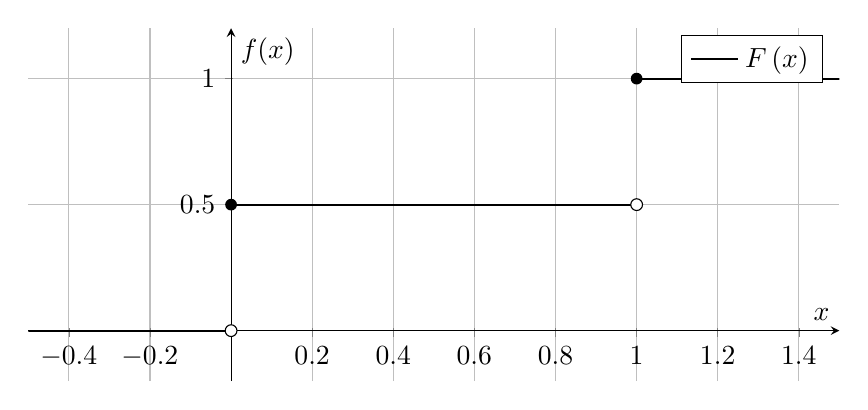
\begin{tikzpicture}
				\begin{axis}[
						tick style = dashed,
						axis lines = {center, left},
						xmin=-0.5, xmax=1.5,
						ymin=-0.2,ymax=1.2,
						grid = major,
						restrict y to domain = -1:3, domain=0:1, width=0.98\textwidth, height=0.5\textwidth, samples=200,  ylabel=$f(x)$, xlabel=$x$, legend entries={$F\left(x\right)$}]
					\addplot[black, thick] {1/2};
					\node at (0,1/2)[circle,fill,inner sep=1.5pt, anchor = center]{};
					\node at (1,1)[circle,fill,inner sep=1.5pt, anchor = center]{};
					\addplot[black, thick, domain = -15:0] {0};
					\addplot[black, thick, domain = 1:15] {1};
					\node at (1,1/2)[circle,draw,fill=white, inner sep=1.5pt, anchor = center]{};
					\node at (0,0)[circle,draw,fill=white,inner sep=1.5pt, anchor = center]{};
				\end{axis}
			\end{tikzpicture}
		\end{center}
	Nota come in questa funzione ogni intervallo $ \left(a,b\right) a,b \in \left[0,1\right)$ abbia probabilità 0! L'intero "peso" si probabilità è contenuto nei singoletti $ \left\{0\right\} $ e $ \left\{1\right\} $
\section{Variabili aleatorie}
Quando effettuiamo un esperimento aleatorio spesso i risultati sono di natura \underline{non numerica}. Spesso tuttavia può essere utile averne di natura numerica. Per soddisfare questa esigenza esistono le \underline{variabili aleatorie}, che permettono di collegare un esito di un esperimento aleatorio di natura non numerica ad un \underline{numero reale}.
Consideriamo il lancio di due dadi a 6 facce. In questo caso avremmo:
\[
	\Omega = \left\{\left(x, y\right) x,y \in 1,\ldots ,6\right\}
\]
tuttavia potrei essere interessato, ad esempio, a trovare la probabilità che \textit{la somma delle due facce sia $ x $}. In questo caso posso usare una variabile aleatoria, che colleghi ogni possibile esito dell'esperimento ad un numero reale (in questo caso ad $ x+y $)
\definizione{Variabile aleatoria}{
	Una \underline{variabile aleatoria reale} $ X $ è una funzione che collega ad ogni elemento di uno spazio campionario $ \Omega $ ad un numero reale:
	\[
		X: \Omega \to \R
	\]
}
inoltre una v.a. può essere discreta o continua
\definizione{V.a. discreta e continua}{
	Una variabile aleatoria si dice:
	\begin{itemize}
		\item \textit{Ddiscreta} se il numero di valori che può assumere è \underline{finito} o \underline{numerabile}
		\item \textit{Continua} se assume un numero di valori \underline{più che numerabile}
	\end{itemize}
}
\subsubsection*{Esempi}
\begin{itemize}
	\item \textit{Discreta} Ad esempio, la variabile che associa al lancio di due dadi la somma dei numero usciti
	\item \textit{Continua} Ad esempio, la variabile che associa al lancio ripetuto 2 volte di una freccetta la somma delle altezze dei due punti colpiti
\end{itemize}
\subsection{Calcolo probabilità tramite v.a.}
Tornando al caso di prima, consideriamo:
\[
	\Omega = \left\{\left(x, y\right) x,y \in 1,\ldots ,6\right\} \quad \mathcal{A} = P\left(\Omega\right)
\]
Definiamo una variabile aleatoria che manda ogni possibile combinazione di dadi nella loro somma:
\[
	X: \Omega \to  \tilde{\Omega } = \left\{2, \ldots ,12\right\}
\]
Se ora volessi calcolare la probabilità che la somma dei lanci sia $ x $, dovrei calcolare la probabilità dell'insieme costituito da tutti gli elementi di omega tali per cui la somma dei due lanci sia $ x $, ossia tutti quelli per cui vale $ X\left(\omega \right) = x \quad \omega  \in \Omega$. Questo insieme chiaramente sta nella tribù scelta ($ \mathcal{A} $)
\[
	Pr\left( \text{somma} = x\right) = Pr\left(\left\{\omega \in \Omega \text{ t.c. } X\left(\omega \right) = x\right\}\right)
\]
Il medesimo discorso può essere fatto se si volesse calcolare la probabilità di un intervallo:
\[
	Pr\left( \text{somma} \in \left(a,b\right] \right) = Pr\left(\left\{\omega \in \Omega \text{ t.c. } a < X\left(\omega \right) \le b \right\}\right)
\]
La per descrivere la distribuzione di una variabile aleatoria può tornare comodo utilizzare un grafico, detto \underline{funzione di probabilità (o densità discreta)}
\definizione{Funzione di probabilità discreta}{
	Sia $ X $ una v.a. e sia $ R_x = \left\{z_1,z_2,\ldots \right\} $ l'insieme di tutti i valori che questa può assumere, allora la funzione seguente definita in $ \R  $ è detta \underline{funzione di probabilità} della v.a. $ X $.
	\[
		\mathrm{p}(x)=
		\begin{cases}
			\Pr\left(X=x_i\right)>0 & x=x_i \in R_X \\
			0                       & x \notin R_X
		\end{cases}
	\]
	$ R_X $ è detto \underline{supporto} della v.a. $ X $
}
\section{Variabili aleatorie discrete}
\subsection{Variabile aleatoria di Bernoulli}
Capita spesso di dover rappresentare un esperimento aleatorio che possa avere due esiti: \underline{successo o insuccesso}. Per modellare questo tipo di scenario è possibile adoperare la v.a. di Bernoulli, che associa ad ogni successo il valore $ 1 $ e ad ogni insuccesso il valore $ 0 $
\definizione{Variabile aleatoria di bernoulli}{
	Una variabile aleatoria di Bernoulli è definita nel seguente modo:
	\[
		x\left(\omega \right)\begin{cases}
			0 & \text{ se insuccesso } \\
			1 & \text{ se successo }
		\end{cases}
	\]
	Nota che $ Pr\left(1\right) = p $, mentre $ Pr\left(0\right) = 1-p $
}
\subsection{Distribuzione binomiale}
\label{vabinomiale} 
\textbox{
	Una distribuzione binomiale esprime il numero di successi ottenuti in $ N $ tentativi
}

Questa distribuzione di probabilità regola il numero dei successi (o risultati favorevoli) conseguito in una successione (finita) di prove indipendenti.
Si supponga che un certo esperimento venga replicato $N \geq 1$ volte e l'esito di ognuno di essi possa essere favorevole (evento $A$ ) oppure non favorevole (evento $A^c$ ). Ad ogni prova dell'esperimento associamo una v.a. $X_i, i=$ $1,2, \cdots, N$ che ne rappresenta l'esito: $X_i=1$ se si verifica $A$ e $X_i=0$ se si verifica $A^c$. Si supponga che le v.a. $X_i, i=1,2, \cdots, N$ siano indipendenti e che $\Pr\left(X_i=1\right)=p, 0 \leq p \leq 1$. Qual è la distribuzione di probabilità del numero totale di successi nelle $N$ prove? Cioè qual è la distribuzione di probabilità della v.a.
\[
	X=X_1+X_2+X_3+\cdots+X_N ?
\]
\definizione{Distribuzione Binomiale}{
	Si dice che una v.a. X si distribuisce secondo la distribuzione di probabilità (o legge) binomiale di parametri $N \geq 1$ (intero) e $ 0 \leq p \leq 1$, se
	\[
		\Pr(X=x)= \begin{cases}
			\binom{N}{x}p^x(1-p)^{N-x} & x=0,1, \cdots, N  \\
			0                          & \text { altrove }\end{cases}
	\]
	e scriveremo $X \sim \operatorname{Bi}(N, p)$.

}
Nel caso speciale in cui $N=1$ la v.a. è chiamata anche v.a. di Bernoulli.
\bigbox{
	La funzione di probabilità del numero totale di successi ottenuti in $N$ prove indipendenti con probabilità di successo pari a $p$ ad ogni prova è dato dalla distribuzione di probabilità di una v.a. binomiale
}
Si consideri una particolare realizzazione per cui il numero di successi è $x$, ad esempio l'allineamento
\[
  B=\{\underbracket[0.1ex]{A, A, \cdots, A}_{x \text { volte }} \underbracket[0.1ex]{A^c, A^c, \cdots, A^c}_{N-x \text { volte }}\}
\]
Poiché le prove sono indipendenti la probabilità di questo allineamento è
\[
	\Pr(B)=p^x(1-p)^{N-x}
\]
e questa è la probabilità di un qualsiasi allineamento con $x$ successi che sono
\[
	\left(\begin{array}{l}
			N \\
			x
		\end{array}\right)
\]
e quindi
\[
	\Pr(X=x)=\left(\begin{array}{l}
			N \\
			x
		\end{array}\right) p^x(1-p)^{N-x}
\]
\teorema{Somma variabili Bernoulliane}{
	Siano $X_1, X_2, \cdots, X_N, N$ v.a. Bernoulliane Bi $(1, p)$ stocasticamente indipendenti allora la v.a. $X$ cosi definita
	\[
		X=\sum_{i=1}^n X_i
	\]
	è tale che $X \sim B i(N, p)$
}
\definizione{Funzione di ripartizione}{
	Sia $ X $ una v.a. Si dice \underline{funzione di ripartizione} della v.a. $ X $ la funzione $ y = F\left(x\right) $ definita per ogni $ x $ reale data da:
	\[
		F\left(x\right) =\Pr\left(X \le x\right) \quad  x \in  \R
	\]
}
Ad esempio, la funzione di ripartizione di una variabile aleatoria che che esprima la somma del lancio di due dadi sarebbe la funzione che in corrispondenza di ogni $ x $ andrebbe esprime la probabilità di ottenere una somma minore di $ x $. Nota che se una v.a. è discreta, posso convertire facilmente da funzione di ripartizione $ F\left(x\right) $ a funzione di probabilità $ p\left(X = x\right) $:
\[
	p\left(X = x\right)  = F\left(x\right) - F\left(x^{-}\right)
\]
dove $ F\left(x^{-}\right) $ è il limite sinistro di $ F $
\vskip3mm
Ad esempio, calcolando la funzione $ f\left(x\right) $ avro che la sua corrispondende funzione di probabilità sarà:
\vskip3mm
\begin{minipage}[t]{0.48\textwidth}
	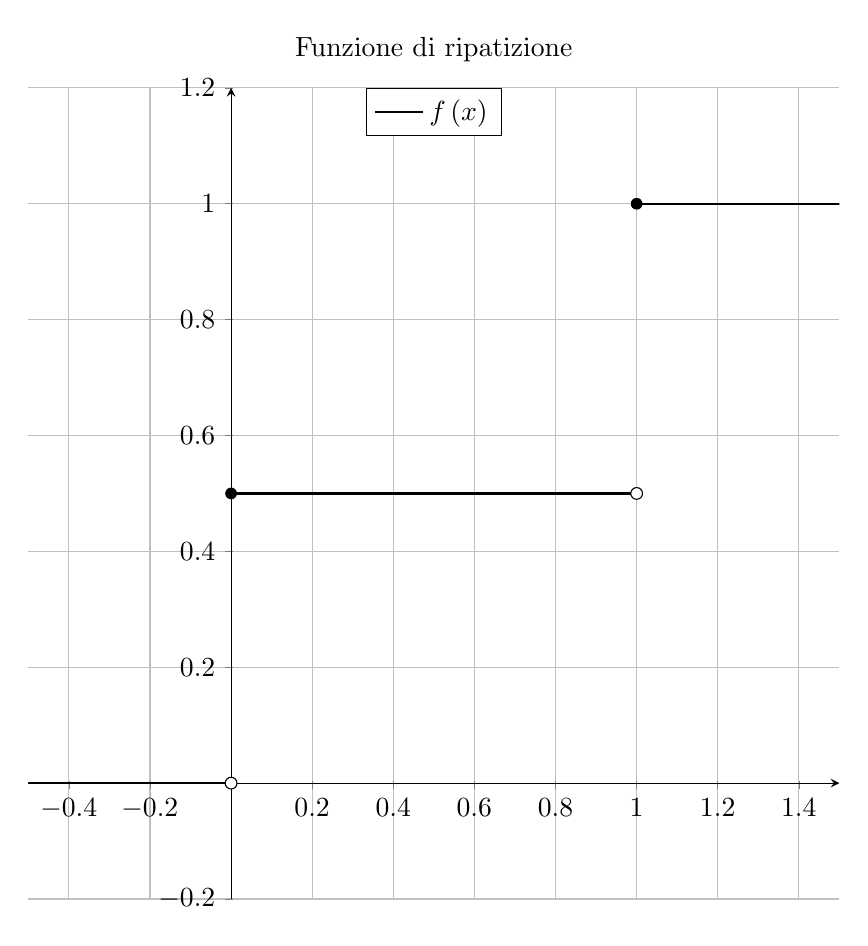
\begin{tikzpicture}
		\begin{axis}[
				title = {Funzione di ripatizione},
				tick style = dashed,
				axis lines = {center, left},
				xmin=-0.5, xmax=1.5,
				ymin=-0.2,ymax=1.2,
				grid = major,
				restrict y to domain = -1:3, domain=0:1, width=0.98\textwidth, height=0.98\textwidth, samples=200, legend entries={$f\left(x\right)$}, legend style = {at = {(0.5, 1)}, anchor = north}]
			\addplot[black, thick] {1/2};
			\node at (0,1/2)[circle,fill,inner sep=1.5pt, anchor = center]{};
			\node at (1,1)[circle,fill,inner sep=1.5pt, anchor = center]{};
			\addplot[black, thick, domain = -15:0] {0};
			\addplot[black, thick, domain = 1:15] {1};
			\node at (1,1/2)[circle,draw,fill=white, inner sep=1.5pt, anchor = center]{};
			\node at (0,0)[circle,draw,fill=white,inner sep=1.5pt, anchor = center]{};
		\end{axis}
	\end{tikzpicture}
\end{minipage}
%
\begin{minipage}[t]{0.48\textwidth}
	\begin{center}
		\begin{tikzpicture}
			\begin{axis}[
					title = {Funzione di probabilità},
					tick style = dashed,
					axis lines = center,
					xmin=-0.5, xmax=1.5,
					ymin=-0.2,ymax=1.2,
					grid = major,
					restrict y to domain = -1:3, domain=0:1, width=0.98\textwidth, height=0.98\textwidth, samples=200, legend entries={$f\left(x\right)$}, legend style = {at = {(0.5, 1)}, anchor = north}]
				\addplot[black, thick, domain = -15:15] {0};
				\node at (0,1/2)[circle,fill,inner sep=1.5pt, anchor = center]{};
				\node at (1,0)[circle,fill=white, draw,inner sep=1.5pt, anchor = center]{};
				\node at (1,1/2)[circle,fill, inner sep=1.5pt, anchor = center]{};
				\node at (0,0)[circle,draw,fill=white,inner sep=1.5pt, anchor = center]{};
				\node at (1/2, 1/2)[whitedot]{};
			\end{axis}
		\end{tikzpicture}
	\end{center}
\end{minipage}
\subsubsection*{Esempi distribuzioni binomiali}
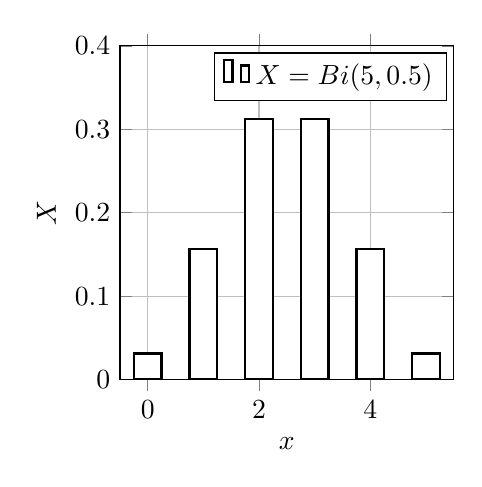
\begin{tikzpicture}
	\begin{axis}[
			xmin=0, xmax=5,
			ymin=0,ymax=0.4,
			ybar,
			enlarge x limits = {0.1},
			restrict y to domain = 0:1, domain=0:5, width=0.48\textwidth, height=0.48\textwidth, grid=major, samples = 6,  ylabel=$X$, xlabel=$x$, legend entries={ {}{$X=Bi(5 ,  0.5) $}}]
		\addplot[black,fill=white, thick] {5!/(x!*(5-x)!)*0.5^x*(1-0.5)^(5-x)};
	\end{axis}
\end{tikzpicture}
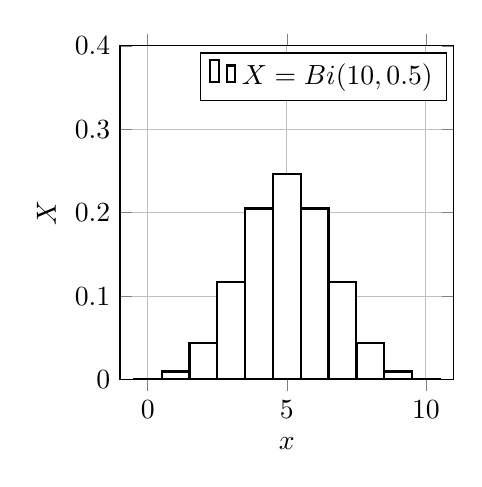
\begin{tikzpicture}
	\begin{axis}[
			xmin=0, xmax=10,
			ymin=0,ymax=0.4,
			ybar,
			enlarge x limits = {0.1},
			restrict y to domain = 0:1, domain=0:10, width=0.48\textwidth, height=0.48\textwidth, grid=major, samples = 11,   ylabel=$X$, xlabel=$x$, legend entries={{}{$X=Bi(10 ,  0.5) $} }]
		\addplot[black,fill=white, thick] {10!/(x!*(10-x)!)*0.5^x*(1-0.5)^(10-x)};
	\end{axis}
\end{tikzpicture}

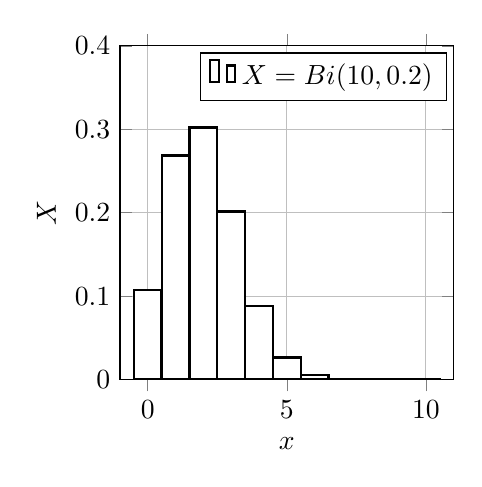
\begin{tikzpicture}
	\begin{axis}[
			xmin=0, xmax=10,
			ymin=0,ymax=0.4,
			ybar,
			enlarge x limits = {0.1},
			restrict y to domain = 0:1, domain=0:10, width=0.48\textwidth, height=0.48\textwidth, grid=major, samples = 11,  ylabel=$X$, xlabel=$x$, legend entries={{}{$X=Bi(10 ,  0.2) $} }]
		\addplot[black,fill=white, thick] {10!/(x!*(10-x)!)*0.2^x*(1-0.2)^(10-x)};
	\end{axis}
\end{tikzpicture}
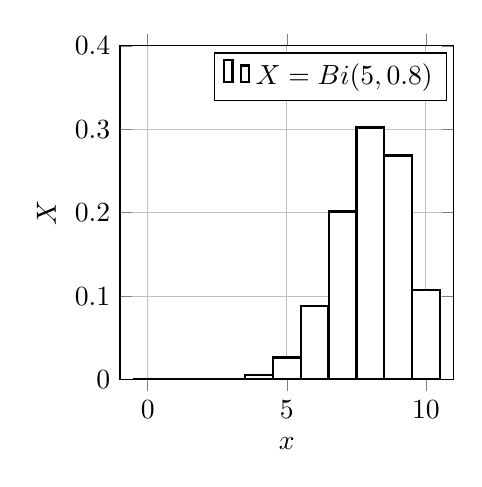
\begin{tikzpicture}
	\begin{axis}[
			xmin=0, xmax=10,
			ymin=0,ymax=0.4,
			ybar,
			enlarge x limits = {0.1},
			restrict y to domain = 0:1, domain=0:10, width=0.48\textwidth, height=0.48\textwidth, grid=major, samples = 11,  ylabel=$X$, xlabel=$x$, legend entries={{}{$X=Bi(5 ,  0.8) $} }]
		\addplot[black,fill=white, thick] {10!/(x!*(10-x)!)*0.8^x*(1-0.8)^(10-x)};
	\end{axis}
\end{tikzpicture}

\begin{tikzpicture}
	\begin{axis}[
			xmin=0, xmax=5,
			ymin=0,ymax=1,
			width=0.48\textwidth, height=0.48\textwidth, grid=major,  ylabel=$X$, xlabel=$x$, declare function={myf(\t)=5!/(\t!*(5-\t)!)*0.5^\t*(1-0.5)^(5-\t);}]
		\addplot [ybar, samples = 6, domain = 0:5, dashed] {myf(x)};
		\draw(0,0)node [whitedot] {}-|
		(1, {myf(1)}) node [whitedot] {} -|% 
		(2, {myf(1) + myf(2)}) node [whitedot] {} -|% 
		(3, {myf(1) + myf(2) + myf(3)}) node [whitedot] {} -|% 
		(4, {myf(1) + myf(2) + myf(3) + myf(4)}) node [whitedot] {} -|% 
		(5, {myf(1) + myf(2) + myf(3) + myf(4) + myf(5)}) node [whitedot] {} -|% 
		(6, {myf(1) + myf(2) + myf(3) + myf(4) + myf(5) + myf(6)}) node [whitedot] {} -|% 
		(7, {myf(1) + myf(2) + myf(3) + myf(4) + myf(5) + myf(6) + myf(7)}) node [whitedot] {} -|% 
		(8, {myf(1) + myf(2) + myf(3) + myf(4) + myf(5) + myf(6) + myf(7) + myf(8)}) node [whitedot] {} -|% 
		(9, {myf(1) + myf(2) + myf(3) + myf(4) + myf(5) + myf(6) + myf(7) + myf(8) + myf(9)}) node [whitedot] {} -|% 
		(10, {myf(1) + myf(2) + myf(3) + myf(4) + myf(5) + myf(6) + myf(7) + myf(8) + myf(9) + myf(10)}) node [whitedot] {};
	\end{axis}
\end{tikzpicture}
\begin{tikzpicture}
	\begin{axis}[
			xmin=0, xmax=10,
			ymin=0,ymax=1,
			width=0.48\textwidth, height=0.48\textwidth, grid=major,  ylabel=$X$, xlabel=$x$, declare function={myf(\t)=10!/(\t!*(10-\t)!)*0.5^\t*(1-0.5)^(10-\t);}]
		\addplot [ybar, samples = 11, domain = 0:10, dashed] {myf(x)};
		\draw(0,0) node [whitedot] {}-|
		(1, {myf(1)}) node [whitedot] {} -|% 
		(2, {myf(1) + myf(2)}) node [whitedot] {} -|% 
		(3, {myf(1) + myf(2) + myf(3)}) node [whitedot] {} -|% 
		(4, {myf(1) + myf(2) + myf(3) + myf(4)}) node [whitedot] {} -|% 
		(5, {myf(1) + myf(2) + myf(3) + myf(4) + myf(5)}) node [whitedot] {} -|% 
		(6, {myf(1) + myf(2) + myf(3) + myf(4) + myf(5) + myf(6)}) node [whitedot] {} -|% 
		(7, {myf(1) + myf(2) + myf(3) + myf(4) + myf(5) + myf(6) + myf(7)}) node [whitedot] {} -|% 
		(8, {myf(1) + myf(2) + myf(3) + myf(4) + myf(5) + myf(6) + myf(7) + myf(8)}) node [whitedot] {} -|% 
		(9, {myf(1) + myf(2) + myf(3) + myf(4) + myf(5) + myf(6) + myf(7) + myf(8) + myf(9)}) node [whitedot] {} -|% 
		(10, {myf(1) + myf(2) + myf(3) + myf(4) + myf(5) + myf(6) + myf(7) + myf(8) + myf(9) + myf(10)}) node [whitedot] {};
	\end{axis}
\end{tikzpicture}

\begin{tikzpicture}
	\begin{axis}[
			xmin=0, xmax=10,
			ymin=0,ymax=1,
			width=0.48\textwidth, height=0.48\textwidth, grid=major,  ylabel=$X$, xlabel=$x$, declare function={myf(\t)=10!/(\t!*(10-\t)!)*0.8^\t*(1-0.8)^(10-\t);}]
		\addplot [ybar, samples = 11, domain = 0:10, dashed] {myf(x)};
		\draw (0,0) node [whitedot]{} -|
		(1, {myf(1)}) node [whitedot] {} -|% 
		(2, {myf(1) + myf(2)}) node [whitedot] {} -|% 
		(3, {myf(1) + myf(2) + myf(3)}) node [whitedot] {} -|% 
		(4, {myf(1) + myf(2) + myf(3) + myf(4)}) node [whitedot] {} -|% 
		(5, {myf(1) + myf(2) + myf(3) + myf(4) + myf(5)}) node [whitedot] {} -|% 
		(6, {myf(1) + myf(2) + myf(3) + myf(4) + myf(5) + myf(6)}) node [whitedot] {} -|% 
		(7, {myf(1) + myf(2) + myf(3) + myf(4) + myf(5) + myf(6) + myf(7)}) node [whitedot] {} -|% 
		(8, {myf(1) + myf(2) + myf(3) + myf(4) + myf(5) + myf(6) + myf(7) + myf(8)}) node [whitedot] {} -|% 
		(9, {myf(1) + myf(2) + myf(3) + myf(4) + myf(5) + myf(6) + myf(7) + myf(8) + myf(9)}) node [whitedot] {} -|% 
		(10, {myf(1) + myf(2) + myf(3) + myf(4) + myf(5) + myf(6) + myf(7) + myf(8) + myf(9) + myf(10)}) node [whitedot] {};
	\end{axis}
\end{tikzpicture}
\begin{tikzpicture}
	\begin{axis}[
			xmin=0, xmax=10,
			ymin=0,ymax=1,
			width=0.48\textwidth, height=0.48\textwidth, grid=major,  ylabel=$X$, xlabel=$x$, declare function={myf(\t)=10!/(\t!*(10-\t)!)*0.2^\t*(1-0.2)^(10-\t);}]
		\addplot [ybar, samples = 11, domain = 0:10, dashed] {myf(x)};
		\draw(0,0) node [whitedot] {}-|
		(1, {myf(1)}) node [whitedot] {} -|% 
		(2, {myf(1) + myf(2)}) node [whitedot] {} -|% 
		(3, {myf(1) + myf(2) + myf(3)}) node [whitedot] {} -|% 
		(4, {myf(1) + myf(2) + myf(3) + myf(4)}) node [whitedot] {} -|% 
		(5, {myf(1) + myf(2) + myf(3) + myf(4) + myf(5)}) node [whitedot] {} -|% 
		(6, {myf(1) + myf(2) + myf(3) + myf(4) + myf(5) + myf(6)}) node [whitedot] {} -|% 
		(7, {myf(1) + myf(2) + myf(3) + myf(4) + myf(5) + myf(6) + myf(7)}) node [whitedot] {} -|% 
		(8, {myf(1) + myf(2) + myf(3) + myf(4) + myf(5) + myf(6) + myf(7) + myf(8)}) node [whitedot] {} -|% 
		(9, {myf(1) + myf(2) + myf(3) + myf(4) + myf(5) + myf(6) + myf(7) + myf(8) + myf(9)}) node [whitedot] {} -|% 
		(10, {myf(1) + myf(2) + myf(3) + myf(4) + myf(5) + myf(6) + myf(7) + myf(8) + myf(9) + myf(10)}) node [whitedot] {};
	\end{axis}
\end{tikzpicture}
%\pgfmathparse{0}
%\pgfmathadd{\pgfmathresult}{1}
%\pgfmathresult
%\pgfmathadd{\pgfmathresult}{1}
%\pgfmathresult
%\pgfmathadd{\pgfmathresult}{1}
%\pgfmathresult
%\pgfmathadd{\pgfmathresult}{1}
%\pgfmathresult
%\pgfmathadd{\pgfmathresult}{1}
%\pgfmathresult
\subsection{Distribuzione geometrica}
\label{vageometrica}
\bigbox{
	\begin{center}
		Una distribuzione geometrica esprime il numero di lanci necessari al fine di ottenere esattamente almeno un successo
	\end{center}
}
Questa distribuzione è simile alla distribuzione binomiale. Anziché contare il numero di successi in $ N $ tentativi, si conta il numero di tentativi prima di ottenere un successo
\begin{table}[h!]
	\centering
	\begin{tabular}{|>{\centering\arraybackslash}p{0.45\textwidth} >{\centering\arraybackslash}p{0.45\textwidth}|}
		\hline
		Variabile binomiale                                                & Variabile geometrica                                                                                 \\
		\hline
		Lanci la moneta $ n $ volte e conti il numero di successi ottenuti & Lanci la moneta \underline{finchè non ottieni} un risultato positivo, e conti quanti lanci hai fatto \\
		\hline
	\end{tabular}
\end{table}
Chiaramente, tutte le prove effettuate devono essere \underline{indipendenti}
\definizione{Distribuzione Geometrica}{
	Si dice che una v.a. $ X $ si distribuisce secondo una distribuzione geometrica di parametro $ 0 \le  p \le  1 $ se la sua funzione di probabilità è :
	\[
		Pr\left(X = x\right) = \begin{cases}
			p\left(1-p\right)^{x-1} & x = 1,2,3,\ldots \\
			0                       & \text{ altrove }
		\end{cases}
	\]
	scriveremo che $ X \sim  Ge \left(P\right) $
}
NB: Talvola la variabile collega il numero di lanci necessari per ottenere un successo ($ n $). Altre volte la variabile collega il numero di insuccessi prima di ottenere un successo ($ n-1 $)
\subsubsection*{Esempi distribuzioni geometriche}
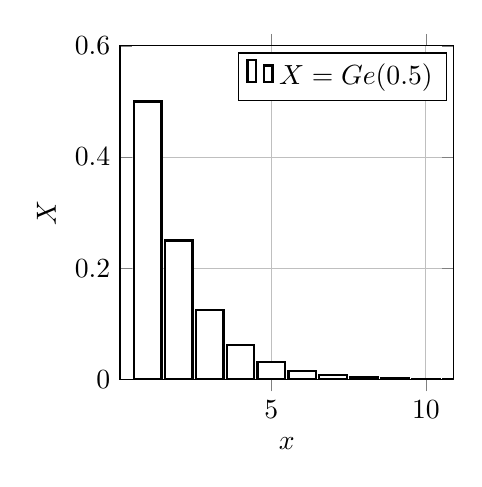
\begin{tikzpicture}
	\begin{axis}[
			xmin=1, xmax=10,
			ymin=0,ymax=0.6,
			ybar,
			enlarge x limits = {0.1},
			domain=1:11, width=0.48\textwidth, height=0.48\textwidth, grid=major, samples = 11,  ylabel=$X$, xlabel=$x$, legend entries={ {}{$X=Ge (0.5)$}}]
		\addplot[black,fill=white, thick] {0.5 * (1-0.5)^(x-1)};
	\end{axis}
\end{tikzpicture}
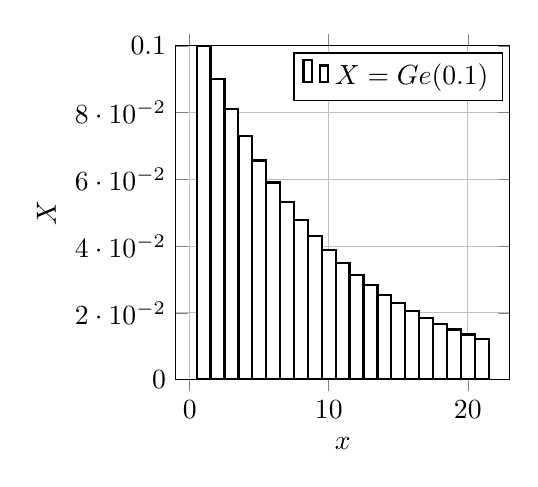
\begin{tikzpicture}
	\begin{axis}[
			xmin=1, xmax=21,
			ymin=0,ymax=0.1,
			ybar,
			bar width = 5pt,
			enlarge x limits = {0.1},
			domain=1:21, width=0.48\textwidth, height=0.48\textwidth, grid=major, samples = 21,  ylabel=$X$, xlabel=$x$, legend entries={ {}{$X=Ge( 0.1) $}}]
		\addplot[black,fill=white, thick] {0.1 * (1-0.1)^(x-1)};
	\end{axis}
\end{tikzpicture}

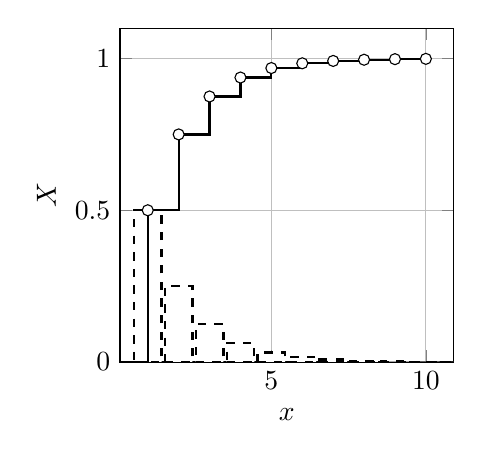
\begin{tikzpicture}
	\begin{axis}[
			xmin=1, xmax=10,
			ymin=0,ymax=1.1,
			enlarge x limits = {0.1},
			domain=1:11, width=0.48\textwidth, height=0.48\textwidth, grid=major, samples = 11,  ylabel=$X$, xlabel=$x$, declare function={myf(\t)=0.5*(1-0.5)^(\t-1);}]
		\addplot[ybar, black,fill=white, thick, dashed] {myf(x)};
		\addplot[const plot, black, thick, domain = 0:10] {0.5 * (1- (1-0.5)^x)/(1-1+0.5)};
		\addplot[const plot,only marks, mark=*, mark options={fill=white}, domain = 0:10] {0.5 * (1- (1-0.5)^x)/(1-1+0.5)};
	\end{axis}
\end{tikzpicture}
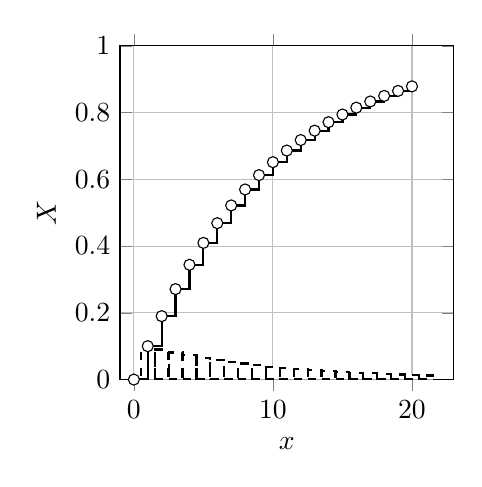
\begin{tikzpicture}
	\begin{axis}[
			xmin=1, xmax=21,
			ymin=0,ymax=1,
			ybar,
			bar width = 5pt,
			enlarge x limits = {0.1},
			domain=1:21, width=0.48\textwidth, height=0.48\textwidth, grid=major, samples = 21,  ylabel=$X$, xlabel=$x$, declare function={myf(\t)=0.1*(1-0.1)^(\t-1);}]
		\addplot[black,fill=white, thick, dashed] {0.1 * (1-0.1)^(x-1)};
		\addplot[const plot, black, thick, domain = 0:20] {0.1 * (1- (1-0.1)^x)/(1-1+0.1)};
		\addplot[const plot,only marks, mark=*, mark options={fill=white}, domain = 0:20] {0.1 * (1- (1-0.1)^x)/(1-1+0.1)};
	\end{axis}
\end{tikzpicture}
\subsection{Distribuzione binomiale negativa}
\bigbox{
	\begin{center}
		Una distribuzione binomiale negativa esprime il numero di lanci necessari al fine di ottenere esattamente $ r $ successi
	\end{center}
}
\definizione{Distribuzione binomiale negativa}{
	Si dice che una v.a. $ X $ si distribuisce secondo la distribuzione binomiale negativa di parametri $ 0 < p \le 1 $ e $ r \ge 1 $ (\underline{intero}) se la sua funzione di probabilità è data da:
	\[
		Pr\left(X = x\right) =
		\begin{cases}
			\binom{x-1}{r-1}p^{r}\left(1-p\right)^{x-1} & x = r, r +1, r+2\ldots \\
			0                                           & \text{ altrove }
		\end{cases}
	\]
	e indichiamo con $ X \sim BinNe\left(r,p\right) $
}
Nota che con $ r = 1 $ la distribuzione coincide con una \underline{variabile geometrica}.
\teorema{Rapporto distribuzione binomiale e binomiale negativa}{
	Sia $ X \sim BiNe\left(r,p\right) $ e $ Z \sim Bi\left(N,p\right) $, allora
	\[
		Pr\left(Z \ge r\right) =\Pr\left(X \le  N\right)
	\]
}
\teorema{Rapporto distribuzione geometrica e binomiale negativa  }{
	Siano $ X_1, X_2,\ldots ,X_r $ delle v.a. \underline{geometriche} stocasticamente indipendenti. Allora la variabile così definita:
	\[
		X = \sum_{i=1}^{r} X_i
	\]
	è una variabile di tipo binomiale negativo: $ X \sim BiNe\left(r,p\right) $
}
 \subsection{Distribuzione di Poisson}
 \label{vapoisson} 
 \bigbox{
   \begin{center}
        Una distribuzione di Poisson esprime il numero di eventi successi in un determinato lasso di tempo/spazio 
   \end{center}
 }
 Ad esempio, una v.a. di Poisson potrebbe eprimere il numero di camion che passano in un'ora su una data strada
\definizione{Distribuzione di Poisson}{
  Si dice che una v.a. $ X $ si distribuisce secondo la distribuzione di Poisson di parametri $ \lambda \ge 0 $ se la sua funzione di probabilità è data da: 
  \[
    \Pr \left(X = x\right) =
    \begin{cases}
    \displaystyle \frac{\lambda ^{x}}{x!} e^{-\lambda } & x \ge 0 \\
    0 & \text{ altrove }
    \end{cases}
  \]
}
\section{Variabili aleatorie continue}
\definizione{Densità di probabilità}{
	se $ F $ è \underline{assolutamente continua} definziamo la \underline{densità} nel seguente modo:
	\[
		f\left(x\right) = F'\left(x\right)
	\]
	Dove $ F\left(x\right) $ è la funzione di ripartizione. Per questa ragione la funzione di ripartizione è una primitiva della funzione di densità. La probabilità di un intervallo $ \left(a, b\right] $ è data da:
	\[
		\int_{a}^{b} f(x) \; dx
	\]
}
Nota che \underline{la funzione di ripartizione è una primitivà della funzione di densità}! L'area del trapezoide della funzione di densità esprime la probabilità del corrispettivo intervallo. La probabilità dell'intervallo $ \left(-\infty, a\right) $ è data da $ \int_{-\infty }^{a} f(x) \; dx $. Tuttavia la probabilità del medesimo intervallo è dato da $ F\left(a\right) $ dove $ F $ è la funzione di ripartizione. Ciò vuol dire che $ F'\left(x\right) = f\left(x\right) $ ossia $ F $ è una primitiva $ f $.
\vskip3mm
\subsubsection*{Esempio funzione di ripartizione e densità}
A sinistra la funzione di ripartizione, a destra la funzione di densità

\begin{minipage}[t]{0.48\textwidth}
	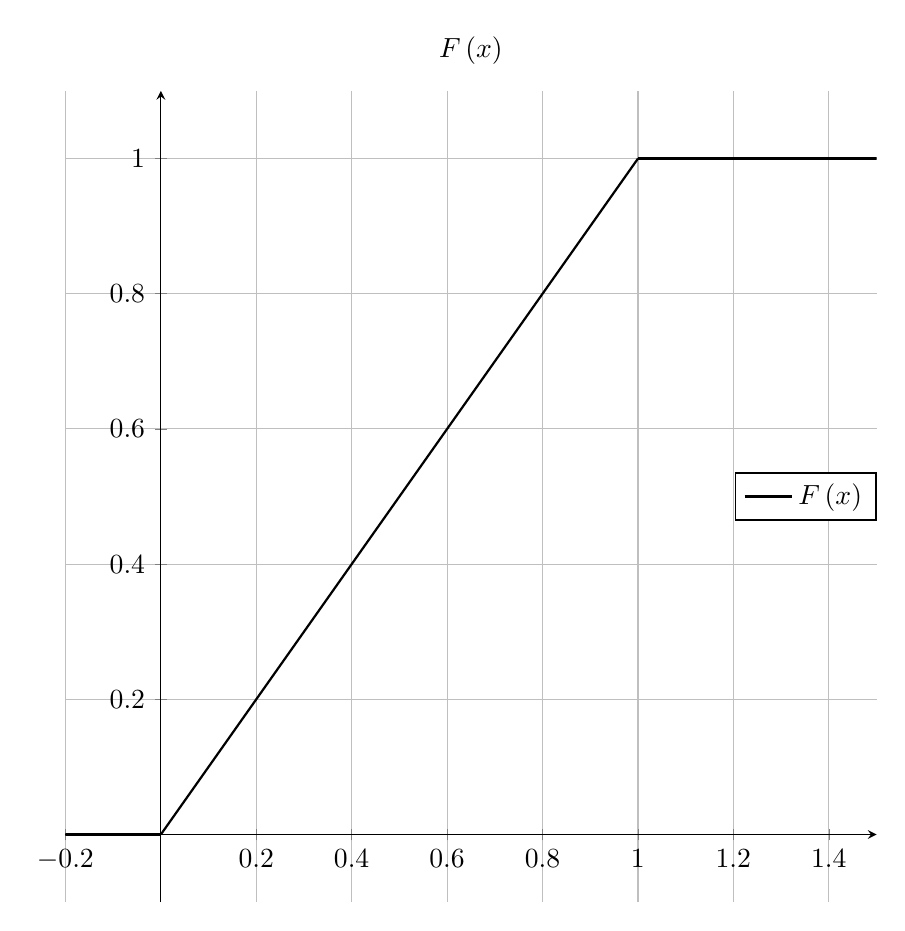
\begin{tikzpicture}
		\begin{axis}[ title = $F\left(x\right)$,
				axis lines = center,
				xmin=-0.2, xmax=1.5,
				ymin=-0.1,ymax=1.1,
				restrict y to domain = -1:3, domain=0:1, width=0.98\textwidth, height=0.98\textwidth, grid=major, samples=200, legend entries={$F\left(x\right)$}, legend style = {anchor = east, at = {(1,0.5)}}]
			\addplot[black, thick] {x};
			\addplot[black, thick, domain = -15:0] {0};
			\addplot[black, thick, domain = 1:15] {1};
		\end{axis}
	\end{tikzpicture}
\end{minipage}
%
\begin{minipage}[t]{0.48\textwidth}
	\begin{center}
		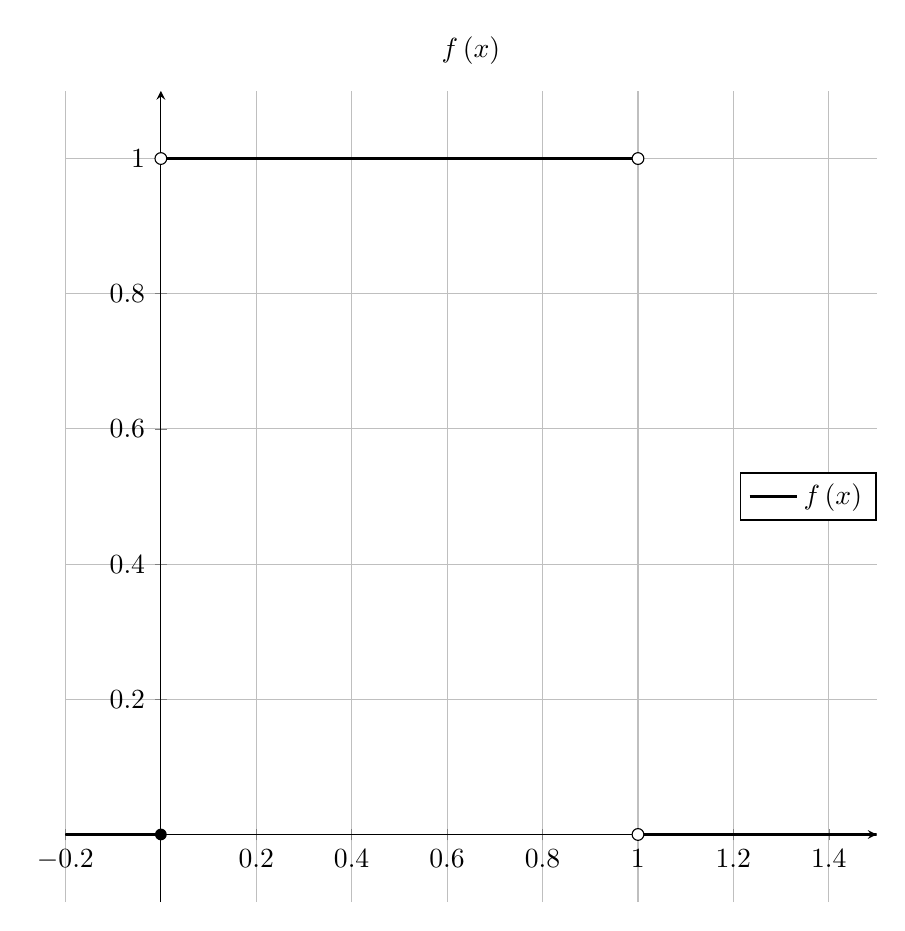
\begin{tikzpicture}
			\begin{axis}[ title = $ f\left(x\right) $,
					axis lines = center,
					xmin=-0.2, xmax=1.5,
					ymin=-0.1,ymax=1.1,
					restrict y to domain = -1:3, domain=0:1, width=0.98\textwidth, height=0.98\textwidth, grid=major, samples=200, legend entries={$f\left(x\right)$}, legend style = {anchor = east, at = {(1,0.5)}}]
				\addplot[black, thick] {1};
				\node at (0,0)[circle,fill,inner sep=1.5pt, anchor = center]{};
				\node at (1,1)[circle,fill,inner sep=1.5pt, anchor = center]{};
				\addplot[black, thick, domain = -15:0] {0};
				\addplot[black, thick, domain = 1:15] {0};
				\node at (1,0)[circle,fill = white, draw,inner sep=1.5pt, anchor = center]{};
				\node at (1,1)[circle,fill = white, draw,inner sep=1.5pt, anchor = center]{};
				\node at (0,1)[circle,fill = white, draw,inner sep=1.5pt, anchor = center]{};
			\end{axis}
		\end{tikzpicture}
	\end{center}
\end{minipage}

\textbox{NB: useremo la teoria dell'integrazione di \underline{Riemann}, ma di solito si userebbe quella di \underline{Lebasgue}}
\subsubsection*{Esempio} Sia $\Omega=[0,1]$ e $\mathcal{A}=\mathcal{B}([0,1])$ la Tribù associata. Sia $\Pr$ la funzione di probabilità su $\mathcal{A}$ definita dalla funzione $F(x)$
\[
	F(x)= \begin{cases}0 & x<0 \\ x & 0 \leq x<1 \\ 1 & x \geq 1\end{cases}
\]
Consideriamo la v.a. $X(\omega)=\omega$ e quindi
\[
	\begin{aligned}
		\Pr(a<X \leq b) & =\Pr(\{\omega \in[0,1]: a<X(\omega) \leq b\})         \\
		                & =\Pr(\{\omega \in[0,1]: a<\omega \leq b\})            \\
		                & =\Pr((a, b])                                          \\
		                & = \begin{cases}b-a=\int_a^b 1 d x & 0 \leq a<b \leq 1 \\
             b                  & a<0<b             \\
             0                  & a<b<0\end{cases}
	\end{aligned}
\]
La v.a. $X$ è dotata di densità
\[
	f(x)= \begin{cases}1 & 0 \leq x \leq 1 \\ 0 & \text { altrove }\end{cases}
\]
\subsubsection*{Esempio 1.2}
Consideriamo sullo stesso spazio la v.a. $Y(\omega)=\omega^2$ allora abbiamo
\[
	\begin{aligned}
		\Pr(a<Y \leq b) & =\Pr(\{\omega \in[0,1]: a<Y(\omega) \leq b\})                                                                                         \\
		                & =\Pr\left(\left\{\omega \in[0,1]: a<\omega^2 \leq b\right\}\right)                                                                    \\
		                & =\Pr(\{\omega \in[0,1]: \sqrt{a}<\omega \leq \sqrt{b}\})                                                                              \\
		                & =\Pr((\sqrt{a}, \sqrt{b}]) \quad= \begin{cases}\sqrt{a}-\sqrt{b}=\int_a^b \frac{1}{2 \sqrt{x}} d x & 0 \leq a<b \leq 1 \\
             \sqrt{b}                                            & a<0<b             \\
             0                                                   & a<b<0\end{cases} \\
		                &
	\end{aligned}
\]
La v.a. $Y$ è dotata di densità
\[
	f(x)= \begin{cases}\frac{1}{2 \sqrt{x}} & 0 \leq x \leq 1 \\ 0 & \text { altrove }\end{cases}
\]
\vskip3mm
%\begin{tikzpicture}
%	\begin{axis}[
%			xmin=-4, xmax=4,
%			ymin=-4,ymax=4,
%			width=0.98\textwidth, height=0.5\textwidth, grid=major, samples=200,  ylabel=$f(x)$, xlabel=$x$]
%		\addplot[black, thick, domain = -15:15] {0};
%		%\coordinate (a) at (1,1/2+3-2+e^0)
%		\coordinate (B) at (2,2);
%		\coordinate (C) at ([shift={(axis direction cs:-2,-2)}] B);
%		\node [blackdot] at (C){};
%		%\draw [-latex](0,0) -- a;
%		%\node [blackdot] at (1,2){};
%	\end{axis}
%\end{tikzpicture}
%
%\begin{tikzpicture}
%	\begin{axis}[
%			xmin=-10, xmax=10,
%			ymin=-40,ymax=40,
%			restrict y to domain =-100:100, domain=-40:40, width=0.48\textwidth, height=0.48\textwidth, grid=major, samples=5000,  ylabel=$f(x)$, xlabel=$x$, legend entries={$ $}, unbounded coords=jump]
%		\addplot[black, thick] {1/sin(deg(x))};
%		\coordinate (B) at (8, {1/sin(deg(8))}) {};
%		\coordinate (A) at (0.75, {1/sin(deg(0.75))}) {};
%		%
%		\draw [dashed] (A)--(B);
%		\node [whitedot] at (5,{sin(deg(5))}){};
%		\node [whitedot] at (B) {};
%		\node [whitedot] at (A) {};
%		%\node [blackdot] at (1,1){};
%	\end{axis}
%\end{tikzpicture}
%\begin{tikzpicture}
%	\begin{axis}[
%			xmin=0, xmax=5,
%			ymin=-4,ymax=4,
%			restrict y to domain = -4:4, domain=0:5, width=0.48\textwidth, height=0.48\textwidth, grid=major, samples=2000,  ylabel=$f(x)$, xlabel=$x$, legend entries={$ $}]
%		\addplot[black, thick] {1/sin(deg(x))};
%		\coordinate (A) at (1, {1/sin(deg(1))}) {};
%		\coordinate (B) at (2.30, {1/sin(deg(2.30))}) {};
%		\coordinate (C) at (3.7, {1/sin(deg(3.7))}) {};
%		\coordinate (D) at (4, {1/sin(deg(4))}) {};
%		%
%		\draw (A) -- (D) {};
%		\draw [dashed] (B) |- (C) {};
%		%
%		\node [whitedot] at (A) {};
%		\node [whitedot] at (B) {};
%		\node [whitedot] at (C) {};
%		\node [whitedot] at (D) {};
%		%
%		%
%		%
%		%
%		%    \node [whitedot] at (intersection of curva1 and curva2){};
%	\end{axis}
%\end{tikzpicture}
%\begin{tikzpicture}
%	\begin{axis}[
%			xmin=-0.5, xmax=1.5,
%			ymin=-1.2,ymax=1.2,
%			restrict y to domain = -1.2:1.2, domain=-0.5:1.5, width=0.48\textwidth, height=0.48\textwidth, grid=major, samples=200,  ylabel=$f(x)$, xlabel=$x$, legend entries={$ $}]
%		\addplot[black, thick] {0};
%		\node [blackdot] at (1,0.5){};
%		\node [blackdot] at (0,1/2){};
%		\node [whitedot] at (1/2,1/2){};
%		\node [whitedot] at (0,0){};
%	\end{axis}
%\end{tikzpicture}
%\begin{tikzpicture}
%	\begin{axis}[
%			xmin=-2, xmax=2,
%			ymin=-2,ymax=2,
%			unbounded coords = jump,
%			restrict y to domain = -4:4, domain=-2:2, width=0.48\textwidth, height=0.48\textwidth, grid=major, samples=200,  ylabel=$f(x)$, xlabel=$x$, legend entries={$ $}]
%		\addplot[black, thick] {e^(-x^2)};
%		\coordinate (A) at (-1, {e^(-(-1)^2)}) {};
%		\coordinate (B) at (-0.5, {e^(-(-0.5)^2)}) {};
%		\coordinate (C) at (0.42, {e^(-0.42^2)}) {};
%		\coordinate (D) at (C|-12,0) {};
%		%\node [whitedot, label=C] at (C) {};
%		\draw [dashed] (A)-|(B);
%		\draw [dashed] (C)--(D);
%		\draw [dotted] (A-|B)--(D);
%		\draw [dotted] (A)|-(D);
%		\node [whitedot] at (A-|B){};
%		%
%		\node [whitedot] at (A) {};
%		\node [outer sep = 5pt, inner sep = 1pt, anchor = south, fill=white] at (A) {A};
%		\node [whitedot] at (B) {};
%		\node [outer sep = 5pt, inner sep = 1pt, anchor = south, fill=white] at (B) {B};
%		\node [whitedot] at (C) {};
%		\node [outer sep = 5pt, inner sep = 1pt, anchor = south, fill=white] at (C) {C};
%		\node [whitedot] at (D) {};
%		\node [outer sep = 5pt, inner sep = 1pt, anchor = south, fill=white] at (D) {D};
%		\node (zero)[whitedot] at (0, {e^(-0^2)}) {};
%		\coordinate (zeroshift) at ([shift={(axis direction cs:0,0.5)}]zero) {};
%		\draw (zero)--(zeroshift);
%		\node [anchor = south, fill=white] at (zeroshift) {\underline{prova}};
%		%\node [whitedot, label=B] at (B) {};
%		%\node [whitedot, label=-90:{}] at (0.42, 0) {};
%		%\node [fill=white, anchor =-90,inner sep = 0pt, outer sep = 5pt] at (0.42, 0) {\underline{prova}};
%		%\node [whitedot] at (A) {};
%	\end{axis}
%\end{tikzpicture}

%\newcommand{\tableline}{
%	\foreach \x in {a,...,z}{
%			\x
%		}
%	\myand
%}
%\def\myvar{}
%\def\height{i}
%\def\width{10}\pgfmathresult
%\pgfmathparse{\width-1}
%prova
%%\pgfmathsetmacro{\width2}{\width -1}
%\foreach \x in {a,...,\height}{
%		\foreach \y in {1,...,\pgfmathresult}{
%				\xappto\myvar{\x \y &}
%			}
%		\xappto\myvar{\x \width \\}
%	}
%\vskip3mm
%\begin{tabular}{|cccccccccc|}
%	\hline
%	\hline
%	\myvar
%	\hline
%	\hline
%\end{tabular}

\subsection{Variabile aleatoria normale o gausiana}
\label{vagaussiana} 
\definizione{V.A. Gaussiana}{
Si diche che una v.a. $ X $ si disttribuisce con legge di probabilità \underline{normale} (o Gaussiana) di parametri:
\begin{itemize}
	\item $ \mu \in \left(-\infty , +\infty \right) $
	\item $ \sigma  \in \left(0, +\infty \right) $
\end{itemize}
se possiede la seguente densità
\[
	f\left(x, \mu , \omega \right) = \frac{1}{\sqrt{2 \pi \sigma ^2 }}e ^{\displaystyle-\frac{1}{2}\frac{\left(x-\mu \right)^2}{\sigma ^2 }}
\]
La indicheremo con $X \sim N \left(\mu , \sigma ^2 \right) $
}
Nota che a differenza delle v.a. discrete, quì stiamo parlando del grafico della \underline{densità} di probabilità, dunque questultima sarà espressa come area del trapezoide sotteso al suo grafico
\textbox{  La variabile $ X \sim N\left(0,1\right) $ è chiamata \textit{Normale standard}}
\subsubsection*{Grafici}
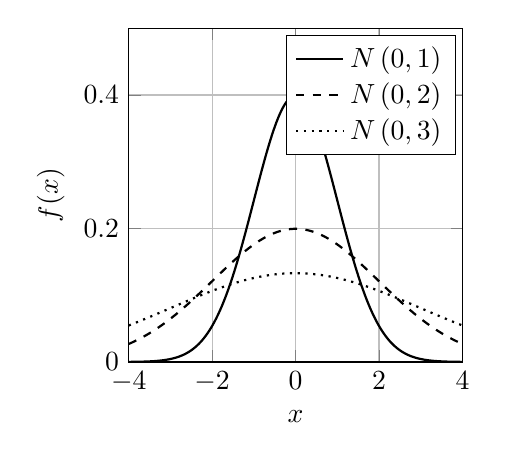
\begin{tikzpicture}
	\begin{axis}[
			xmin=-4, xmax=4,
			ymin=0,ymax=0.5,
			restrict y to domain = 0:0.5, domain=-4:4, width=0.48\textwidth, height=0.48\textwidth, grid=major, samples=200,  ylabel=$f(x)$, xlabel=$x$, legend entries={{}{$N\left(0,1\right)$}, {$ N\left(0,2\right) $}, {$ N\left(0,3\right) $}}]
		\def\myomega{1}
		\def\mymu{0}
		\addplot[black, thick] {1/(sqrt(2*pi*\myomega^2))*e^(-1/2*((x-\mymu)^2)/(\myomega^2))};
		\def\myomega{2}
		\addplot[black, thick, dashed] {1/(sqrt(2*pi*\myomega^2))*e^(-1/2*((x-\mymu)^2)/(\myomega^2))};
		\def\myomega{3}
		\addplot[black, thick, dotted] {1/(sqrt(2*pi*\myomega^2))*e^(-1/2*((x-\mymu)^2)/(\myomega^2))};
	\end{axis}
\end{tikzpicture}
%
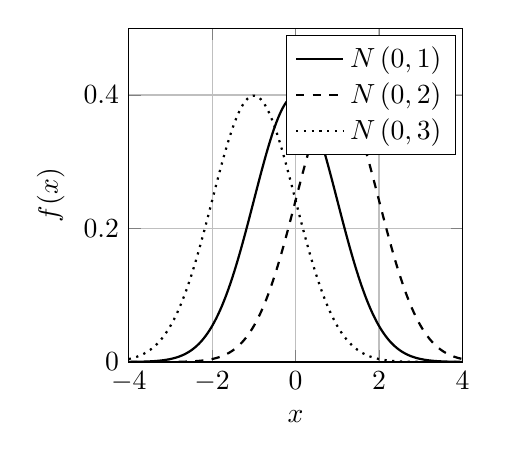
\begin{tikzpicture}
	\begin{axis}[
			xmin=-4, xmax=4,
			ymin=0,ymax=0.5,
			restrict y to domain = 0:0.5, domain=-4:4, width=0.48\textwidth, height=0.48\textwidth, grid=major, samples=200,  ylabel=$f(x)$, xlabel=$x$, legend entries={{}{$N\left(0,1\right)$}, {$ N\left(0,2\right) $}, {$ N\left(0,3\right) $}}]
		\def\myomega{1}
		\def\mymu{0}
		\addplot[black, thick] {1/(sqrt(2*pi*\myomega^2))*e^(-1/2*((x-\mymu)^2)/(\myomega^2))};
		\def\mymu{1}
		\addplot[black, thick, dashed] {1/(sqrt(2*pi*\myomega^2))*e^(-1/2*((x-\mymu)^2)/(\myomega^2))};
		\def\mymu{-1}
		\addplot[black, thick, dotted] {1/(sqrt(2*pi*\myomega^2))*e^(-1/2*((x-\mymu)^2)/(\myomega^2))};
	\end{axis}
\end{tikzpicture}


Come è possibile osservare $ \mu   $ determina il valore al quale è situato il picco della densità, mentre $ \sigma  $ regola quanto i risultati sono concentrati intorno a questo picco
%\begin{tikzpicture}
%  \begin{axis}[
%  xmin=-4, xmax=4,
%  ymin=0,ymax=2,
%  restrict y to domain = 0:2, domain=-4:4, width=0.98\textwidth, height=0.5\textwidth, grid=major, samples=200,  ylabel=$f(x)$, xlabel=$x$, legend entries={$ $}]
%%\addplot[black, thick] {1/(2*pi*2)*e^(-0.5*((x-0)^2)/2)};
%\addplot[black, thick] {2*x}
%  \end{axis}
%\end{tikzpicture}
\subsubsection*{Normalizzazione}
Visto che la funzione di densità della v.a. \textit{Gaussiana} non è integrabile in forma chiusa, sono disponibili delle tabelle che approssimano l'integrale della normale standard in determinati suoi punti. Se la nostra v.a. non è standard, dobbiamo applicare il processo di normalizzazione. Si può dimostrare che
\[
	Z = \frac{ X - \mu }{\sigma } \sim  N \left(0,1\right)
\]
ossia $ Z $ è una normale standard
Per questa ragione possiamo trasformare la nostra v.a. in una normale standard e calcolare l'area di nostro gradimento:
\[
	\Pr \left(\left\{ X \le  c\right\}\right) = \Pr \left(\left\{\frac{ X - \mu }{\sigma }\le  \frac{ c - \mu  }{\sigma }\right\}\right)
\]
\begin{itemize}
	\item Voglio calcolare $ \Pr\left(X \le c\right) $
	\item Calcolo $ \frac{c -\mu }{\sigma } $
	\item Vedo sulla tabella l'area della normale standard nell'intervallo $ \left(-\infty \frac{ c - \mu }{\sigma }\right] $
\end{itemize}
\subsection{Distribuzione Esponenziale}
\label{vaesponenziale} 
\definizione{Distribuzione esponenziale}{
	Si diche che una v.a. $ X $ ha \underline{legge esponenziale} con parametro $  \lambda > 0 $ se la sua funzione di densità ha la forma:
	\[
		f\left(x;
		\lambda \right) = \begin{cases}
			\lambda e^{ -\lambda  x} & x > 0           \\
			0                        & \text{altrove }
		\end{cases}
	\]
	e la  indichiamo nel seguente modo $  X \sim \operatorname{Exp}\left(\lambda\right) $
}
A differenza della v.a. Gaussiana, in questo caso è possibile ricavare l'espressione esplicita della funzione di ripartizione:
\[
	F\left(x\right) =
	\begin{cases}
		\int_{0}^{x} \lambda  e ^{ -\lambda t} \; dt = 1 - e^{ -\lambda  x} & x \ge  0 \\
		0                                                                   & x < 0
	\end{cases}
\]
\textbox{Come la \textit{distribuzione geometrica}, anche quella esponenziale \underline{non ha memoria}}
\[
	\begin{aligned}
		\Pr(y<X \leq y+x \mid X>y) & =\frac{\Pr(\{y<X \leq y+x\} \cap\{X>y\})}{\Pr(\{X>y\})}  \\
		                           & =\frac{\Pr(\{y<X \leq y+x\})}{\Pr(\{X>y\})}              \\
		                           & =\frac{e^{-\lambda y}-e^{-\lambda(y+x)}}{e^{-\lambda y}} \\
		                           & =1-e^{-\lambda x}=\Pr(X \leq x)
	\end{aligned}
\]
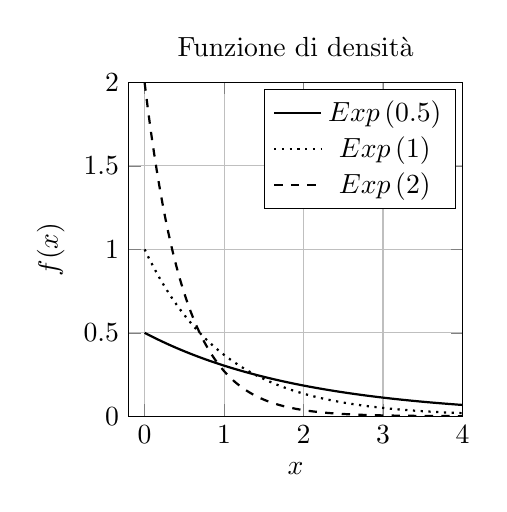
\begin{tikzpicture}
	\begin{axis}[title ={Funzione di densità},
			xmin=-0.2, xmax=4,
			ymin=0,ymax=2,
			restrict y to domain = -1:2, domain=0:4, width=0.48\textwidth, height=0.48\textwidth, grid=major, samples=200,  ylabel=$f(x)$, xlabel=$x$, legend entries={$\operatorname{Exp}\left(0.5\right) $, $\operatorname{Exp}\left(1\right) $, $\operatorname{Exp}\left(2\right) $}]
		\addplot[black, thick] {0.5*e^(-1/2*x)};
		\addplot[dotted, thick] {1*e^(-1*x)};
		\addplot[dashed, thick] {2*e^(-2*x)};
	\end{axis}
\end{tikzpicture}
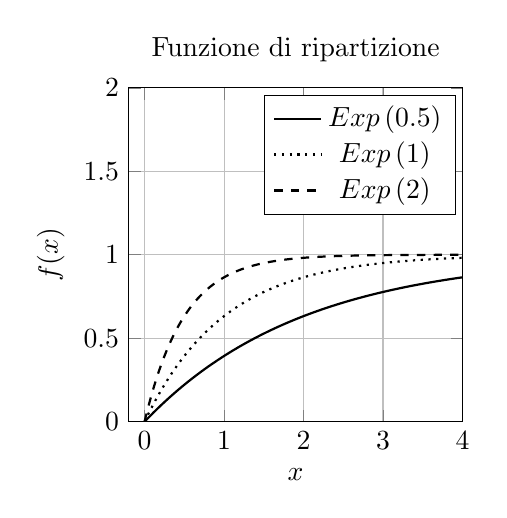
\begin{tikzpicture}
	\begin{axis}[title ={Funzione di ripartizione},
			xmin=-0.2, xmax=4,
			ymin=0,ymax=2,
			restrict y to domain = -1:2, domain=0:4, width=0.48\textwidth, height=0.48\textwidth, grid=major, samples=200,  ylabel=$f(x)$, xlabel=$x$, legend entries={$\operatorname{Exp}\left(0.5\right) $, $\operatorname{Exp}\left(1\right) $, $\operatorname{Exp}\left(2\right) $}]
		\addplot[black, thick] {1-e^(-0.5*x)};
		\addplot[dotted, thick] {1-e^(-1*x)};
		\addplot[dashed, thick] {1-e^(-2*x)};
	\end{axis}
\end{tikzpicture}

\subsection{Cheatsheet e cose che non ho voglia di dimostrare}
\begin{table}[h!]
	\centering
	\begin{tabular}{|c c c|}
		\hline
		Variabile                                                         & Media                               & Varianza                               \\
		\hline
    \textit{Bernoulli} $ \mathcal{B} \left(p\right) $ & p & $ p \left(1-p\right) $ \\
		\textit{Binomiale} $ Bi\left(N, p\right) $                        & $ N p $                             & $ Np \left(1-p\right) $                \\
		\textit{Geometrica} $ \operatorname{Ge}\left(p\right) $            & $\displaystyle  \frac{1}{p} $       & $\displaystyle  \frac{1-p}{p^2 } $     \\
        \textit{Poisson} $ \mathcal{P} \left(\lambda \right) $ & $ \lambda  $ & $ \lambda $ \\
		\textit{Normale} $\displaystyle \mathcal{N} \left(\mu , \sigma ^2 \right) $ & $\displaystyle \mu  $               & $\displaystyle \sigma ^2  $             \\
    \textit{Esponenziale} $ \displaystyle   \operatorname{Exp}\left(\lambda \right) $  & $\displaystyle \frac{1}{\lambda } $ & $\displaystyle \frac{1}{\lambda ^2 } $ \\
		\hline
	\end{tabular}
\end{table}
\section{Scale di misura, moda, quantili, momenti}
\subsection{Trasformazioni variabili aleatorie}
Per alterare come una variabile aleatoria si distribuisce è possibile utilizzare le trasformazioni. Una trasformazione non è altro che una funzione che viene applicata al valore assunto dalla variabile aleatoria. Ad esempio, se condideriamo la funzione $ g\left(x\right) = x + 2 $ e consideriamo:
\[
	\omega = \left\{\text{ rosso }, \text{ verde }, \text{ azzurro }\right\}
\]
\[
	X\left(\text{rosso}\right)=1  \quad X \left(\text{verde}\right) = 2 \quad X \left(\text{azzurro}\right) = 3
\]
possiamo applicare la funzione $ g\left(x\right) $ sulla variabile aleatoria $ X $ per ottenere un'altra variabile aleatoria $ Y $:
\begin{align*}
	 & Y\left(\text{rosso}\right)=g\left(X\left(\text{rosso}\right)\right) = g\left(1\right) = 1 + 2 = 3     \\
	 & Y\left(\text{verde}\right)=g\left(X\left(\text{verde}\right)\right) = g\left(2\right) = 2 + 2 = 4     \\
	 & Y\left(\text{azzurro}\right)=g\left(X\left(\text{azzurro}\right)\right) = g\left(3\right) = 3 + 2 = 5
\end{align*}
Supponendo che la variabile $ X $ si distribuisca come qui a sinistra, la variabile $ Y $ si distribuirebbe come qui a destra:
\vskip3mm
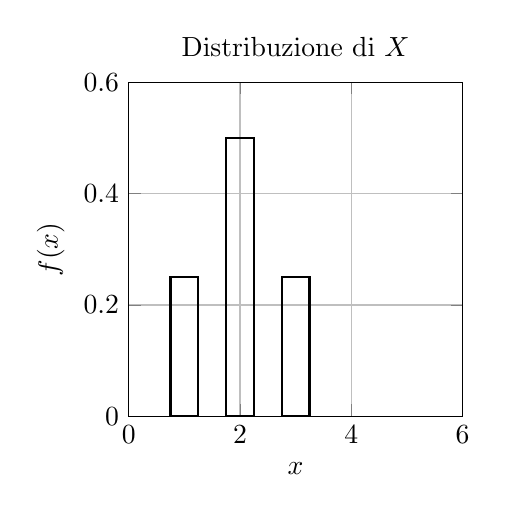
\begin{tikzpicture}
	\begin{axis}[
			title = {Distribuzione di $ X $},
			xmin=0, xmax=6,
			ymin=0,ymax=0.6,
			restrict y to domain = 0:1, domain=0:5, width=0.48\textwidth, height=0.48\textwidth, grid=major, samples=200,  ylabel=$f(x)$, xlabel=$x$]
		\addplot[black, thick, ybar] coordinates{(1,0.25) (2, 0.5) (3, 0.25)};
	\end{axis}
\end{tikzpicture}
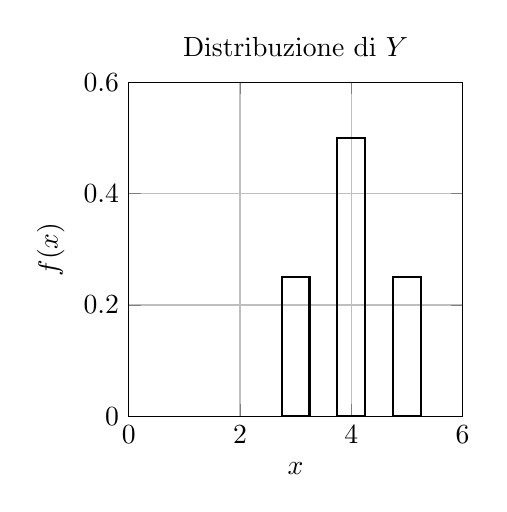
\begin{tikzpicture}
	\begin{axis}[
			title = {Distribuzione di $ Y $},
			xmin=0, xmax=6,
			ymin=0,ymax=0.6,
			restrict y to domain = 0:1, domain=0:5, width=0.48\textwidth, height=0.48\textwidth, grid=major, samples=200,  ylabel=$f(x)$, xlabel=$x$]
		\addplot[black, thick, ybar] coordinates{(3,0.25) (4, 0.5) (5, 0.25)};
	\end{axis}
\end{tikzpicture}


Non tutte le funzioni possono essere applicate come trasformazioni, in quanto deve essere possibile calcolare la probabilità su ogni valore assunto dalla variabile $ Y $ trasformata. Per fare ciò è necessario dover poter calcolare la probabilità sul suo insieme controimmagine sei valori assunti da $ X $ in corrispondenza del valore assunto da $ Y $. Formalmente:
\definizione{Traformazione di una v.a.}{
	Consideriamo una funzione $  Y \left(\omega \right) = g\left(X \left(\omega \right)\right) $ dove $ g : \R  \to  \R  $. Se $ g $ è tale che
	\[
		\left\{ x \in  \R  : g\left(x\right) \le  z \right\} \in  \mathcal{B}\left(\R \right)\text{ per ogni }z \in  \R
	\]
	allora $ Y\left(\omega \right) $ è una variabile aleatoria
}
visto che è difficile verificare se questa condizione è verificata, noi useremo il seguente teorema:
\teorema{Funzioni utilizzabili per trasformazioni v.a.}{
	Una funzione $ g\left(x\right) $ può essere utilizzata per effettuare una trasformazione di una v.a. se soddifa almeno una delle seguenti conidizoni:
	\begin{itemize}
		\item \underline{Continuità}
		\item \underline{Monotonia} (\textit{crescente o decrescente})
	\end{itemize}
}
\label{requisiti trasformazione}
Quindi formalmente, se poniamo:
\[
	A \left(y\right) = \left\{ x \in  \R : g\left(x\right) \le  y\right\}
\]
allora abbiamo
\[
	\Pr(Y(\omega) \leq y)=\Pr(X(\omega) \in A(y))
\]
Nel caso discreto abbiamo:
\[
	\Pr(Y \leq y)=\sum_{\{x: g(x) \leq y\}} p_X(x)
\]
mentre nel caso di una v.a. dotata di densità
\[
	\Pr(Y \leq y)=\int_{\{x: g(x) \leq y\}} f_X(x) d x
\]
\teorema{Densità di v.a. trasformata}{
	Sia $X$ una v.a. con densità $f_X(x)$ con supporto l'intervallo $(a, b)$, eventualmente non limitato. Sia $g(x)$ una funzione strettamente monotona con derivata in $(a, b)$.
	Allora la v.a. $Y=g(X)$ è dotata di densità
	\[
		f_Y(y)= \begin{cases}f_X\left(g^{-1}(y)\right)\left|D\left[g^{-1}(y)\right]\right| & \alpha<y<\beta \\ 0 & \text { altrove }\end{cases}
	\]
	dove $\alpha=\min (g(a), g(b))$ e $\beta=\max (g(a), g(b))$.
}
\label{trasformazioni}
\subsubsection*{Esempio}
Sia $X$ una v.a. esponenziale di parametro $\lambda$. Sia $g(x)=e^x$. Allora applicando il teorema precedente abbiamo
\begin{itemize}
	\item $\alpha=g(a)=g(0)=1$
	\item $\beta=g(b)=g(+\infty)=+\infty$
	\item $g^{-1}(y)=\log (y)$ per $1<y<+\infty$
	\item $D \left[g^{-1}(y)\right]=\frac{1}{y}$
\end{itemize}
allora
\[
	f_Y(y)=\lambda \exp (-\lambda \log (y)) \frac{1}{y}=\frac{\lambda}{y^{\lambda+1}} \quad 1<y<+\infty
\]
e 0 altrove.
\vskip3mm
Esempio di una trasformazione di una variabile $ X \sim N\left(0,1\right) $ tramite la funzione $ g\left(x\right) = 2x $

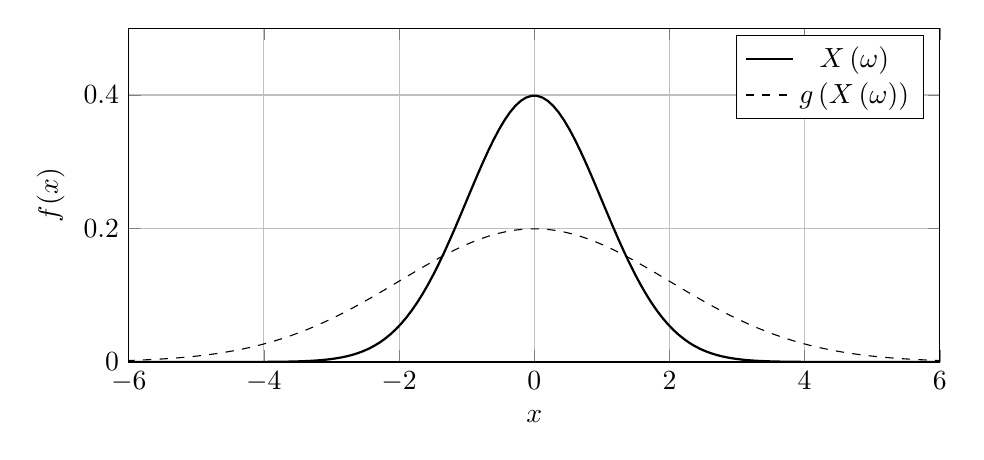
\begin{tikzpicture}
	\begin{axis}[
			xmin=-6, xmax=6,
			ymin=0,ymax=0.5,
			restrict y to domain = 0:0.5, domain=-8:8, width=0.98\textwidth, height=0.48\textwidth, grid=major, samples=200,  ylabel=$f(x)$, xlabel=$x$, legend entries={{}{$X\left(\omega \right)$}, {$ g\left(X\left(\omega \right)\right) $}}]
		\def\myomega{1}
		\def\mymu{0}
		\addplot[black, thick] {1/(sqrt(2*pi*\myomega^2))*e^(-1/2*((x-\mymu)^2)/(\myomega^2))};
		\addplot[black, dashed] {1/2*1/(sqrt(2*pi*\myomega^2))*e^(-1/2*((1/2*x-\mymu)^2)/(\myomega^2))};
	\end{axis}
\end{tikzpicture}

\subsubsection*{Quando il teorema sulle trasformazioni non può essere applicato}
Prendiamo come esempio la v.a.
\[
	X \sim N\left(0,1\right)
\]
ossia una \textit{normale standard}.
Quando la funzione per la quale non è monotona o non ha derivata in un determinato intervallo è possibile comunque calcolarne la probabilità in altri modi. Vediamo un esempio interessante. In seguito affronteremo i momenti. Il momento di ordine $ \alpha $ di una v.a. è così definito:
\[
	u_1=\mathbb{E}\left(X^2 \right)
\]
Tuttavia non si può appicare il teorema \ref{trasformazioni} per trasformare una v.a. tramite la funzione $ g\left(x\right) = x^2  $, in quanto la funzione $ g\left(x\right) $ \underline{non è monotona}. Tuttavia, possiamo tenere in mente che:
\begin{itemize}
	\item La probabilità di un intervallo $ \left(a,b\right] $ di una variabile trasformata $ X' $ è uguale alla probabilità della controimmagine dell'intervallo $ \left(a,b\right] $ della variabile $ X $
	\item E' possibile ricavare l'intervallo controimmagine tramite una semplice disequazione, quindi:
	      \begin{align*}
		      Pr\left(X' < a\right) =\Pr\left(X^2 < a\right) =\Pr\left(X \in \left(-\sqrt{a}, \sqrt{a}\right)\right) = \int_{-\sqrt{a}}^{\sqrt{a}} f(x) \; dx
	      \end{align*}
	\item Per calcolare la forma esplicita della distribuzione della variabile $ X' $ posso procedere come segue:
	      \begin{align*}
		      F_{X'} \left(a\right) & =\Pr\left(X' < a\right) =\Pr\left(X^2 < a\right) =\Pr\left(X \in \left(-\sqrt{a}, \sqrt{a}\right)\right) \\
		                            & =2 \int_{0}^{\sqrt{a}} f(x) \; dx
	      \end{align*}
	      dove $ f\left(x\right) $ è la distribuzione di $ X $. Nota che l'ultima eguaglianza è data dal fatto che la funzione di distribuzione di una normale standard è \underline{pari}
	\item Sapendo che $ f_{X'}\left(x\right) $, ossia la distribuzione di $ X' $ è la derivata della sua funzione di ripartizione:
	      \begin{align*}
		      f_{X'}\left(a\right) & = D\left[f_{X'}\left(a\right)\right]= D\left[2 \int_{0}^{\sqrt{a}} f(x) \; dx\right] \\
		                           & = \frac{f\left(\sqrt{a}\right)}{\sqrt{a}}
	      \end{align*}
\end{itemize}
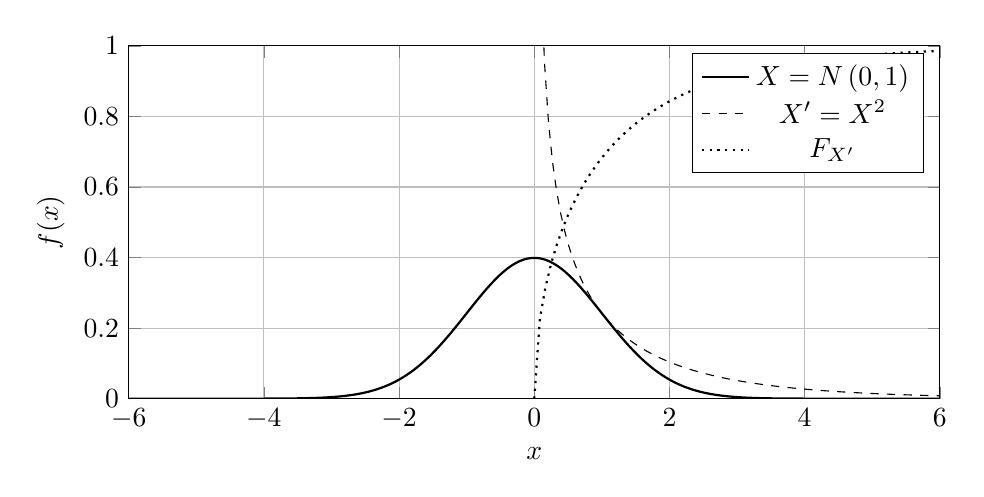
\begin{tikzpicture}
	\begin{axis}[
			xmin=-6, xmax=6,
			ymin=0,ymax=1,
			restrict y to domain = 0:6, domain=-6:6, width=0.98\textwidth, height=0.5\textwidth, grid=major, samples=200,  ylabel=$f(x)$, xlabel=$x$, legend entries={{}{$ X=N\left(0,1\right) $}, {$ X' = X^2  $}, {$F_{X'}$}}, declare function = {f(\x)=1/sqrt(2*pi)*e^(-1/2*\x^2);}]
		\addplot[black, thick] {f(x)};
		\addplot[black, dashed] {f(sqrt(x))/sqrt(x)};
		\addplot [dotted, thick] coordinates {(0,0) (0.08270009615900084,0.22632886848699163) (0.16540009591800084,0.31576733009822505) (0.24810009567700084,0.381583953083551) (0.33080009543600086,0.4348116577210977) (0.41350009519500086,0.4798016799958162) (0.49620009495400086,0.5188254571101616) (0.5789000947130009,0.5532562280994735) (0.6616000944720009,0.5840043824857597) (0.7443000942310009,0.6117131230740239) (0.8270000939900009,0.6368585800675296) (0.9097000937490008,0.659805994810897) (0.9924000935080008,0.6808435226421935) (1.0751000932670007,0.7002037095958256) (1.1578000930260006,0.7180777505853322) (1.2405000927850005,0.7346253044828348) (1.3232000925440004,0.749981459286068) (1.4059000923030003,0.7642618046313453) (1.4886000920620002,0.7775662094565895) (1.571300091821,0.7899816907127856) (1.65400009158,0.8015846294962505) (1.7367000913389998,0.8124425092698303) (1.8194000910979997,0.8226152978567983) (1.9021000908569996,0.8321565596789661) (1.9848000906159995,0.8411143607915674) (2.0675000903749994,0.8495320126974736) (2.1502000901339993,0.8574486892386244) (2.232900089892999,0.8648999424890241) (2.315600089651999,0.8719181374839694) (2.398300089410999,0.878532821131383) (2.481000089169999,0.8847710373010664) (2.5637000889289987,0.8906575975587295) (2.6464000886879986,0.8962153150821911) (2.7291000884469985,0.901465207810528) (2.8118000882059984,0.9064266757209585) (2.8945000879649982,0.9111176562216702) (2.977200087723998,0.9155547609320581) (3.059900087482998,0.9197533965509299) (3.142600087241998,0.9237278720552858) (3.225300087000998,0.9274914941024244) (3.3080000867599977,0.9310566522076136) (3.3907000865189976,0.934434895023882) (3.4734000862779975,0.9376369988485291) (3.5561000860369973,0.9406730293140417) (3.6388000857959972,0.9435523970824554) (3.721500085554997,0.9462839082464907) (3.804200085313997,0.9488758100437503) (3.886900085072997,0.9513358324085676) (3.969600084831997,0.9536712258169773) (4.052300084590997,0.9558887958216301) (4.135000084349997,0.9579949346234516) (4.217700084108997,0.9599956499840923) (4.300400083867997,0.961896591746488) (4.383100083626997,0.9637030761992432) (4.4658000833859965,0.9654201084932243) (4.548500083144996,0.9670524032950729) (4.631200082903996,0.9686044038417729) (4.713900082662996,0.9700802995424604) (4.796600082421996,0.9714840422579806) (4.879300082180996,0.9728193613749576) (4.962000081939996,0.9740897777790605) (5.044700081698996,0.975298616821511) (5.127400081457996,0.9764490203634895) (5.2101000812169955,0.9775439579747822) (5.292800080975995,0.97858623735564) (5.375500080734995,0.9795785140442704) (5.458200080493995,0.980523300466549) (5.540900080252995,0.9814229743793284) (5.623600080011995,0.9822797867540701) (5.706300079770995,0.9830958691433538) (5.789000079529995,0.9838732405690751) (5.871700079288995,0.984613813967784) (5.9544000790479945,0.9853194022255822) (6.037100078806994,0.98599172383227) (6.119800078565994,0.986632408181964) (6.202500078324994,0.9872430005451766) (6.285200078083994,0.9878249667353224) (6.367900077842994,0.9883796974907869) (6.450600077601994,0.9889085125920184) (6.533300077360994,0.9894126647315956) (6.616000077119994,0.989893343153833) (6.6987000768789935,0.9903516770792318) (6.781400076637993,0.9907887389279291) (6.864100076396993,0.9912055473552485) (6.946800076155993,0.9916030701114867) (7.029500075914993,0.991982226737195) (7.112200075673993,0.9923438911043952) (7.194900075432993,0.9926888938134333) (7.277600075191993,0.9930180244544855) (7.360300074950993,0.9933320337421031) (7.4430000747099925,0.9936316355306022) (7.525700074468992,0.9939175087175692) (7.608400074227992,0.9941902990422616) (7.691100073986992,0.9944506207852237) (7.773800073745992,0.9946990583750194) (7.856500073504992,0.9949361679075927) (7.939200073263992,0.9951624785834038) (8.021900073022993,0.9953784940671577) (8.104600072781993,0.9955846937746278) (8.187300072540994,0.9957815340907921) (8.270000072299995,0.9959694495232304) (8.352700072058996,0.996148853794483) (8.435400071817996,0.9963201408768386) (8.518100071576997,0.9964836859728075) (8.600800071335998,0.9966398464443289) (8.683500071094999,0.9967889626935851) (8.766200070854,0.9969313589981068) (8.848900070613,0.9970673443027066) (8.931600070372001,0.9971972129706128) (9.014300070131002,0.9973212454960433) (9.097000069890003,0.9974397091803218) (9.179700069649003,0.9975528587735151) (9.262400069408004,0.9976609370834589) (9.345100069167005,0.9977641755539232) (9.427800068926006,0.997862794813574) (9.510500068685007,0.9979570051972907) (9.593200068444007,0.9980470072413058) (9.675900068203008,0.9981329921535558) (9.758600067962009,0.9982151422605489) (9.84130006772101,0.9982936314319849) (9.92400006748001,0.9983686254842896) (10.006700067239011,0.9984402825641665) (10.089400066998012,0.9985087535132011) (10.172100066757013,0.9985741822145022) (10.254800066516014,0.9986367059223047) (10.337500066275014,0.998696455575412) (10.420200066034015,0.9987535560953072) (10.502900065793016,0.9988081266697146) (10.585600065552017,0.9988602810223544) (10.668300065311017,0.9989101276695926) (10.751000065070018,0.9989577701646484) (10.833700064829019,0.9990033073299879) (10.91640006458802,0.9990468334784999) (10.99910006434702,0.999088438624016) (11.081800064106021,0.9991282086817092) (11.164500063865022,0.9991662256588763) (11.247200063624023,0.9992025678365839) (11.329900063383024,0.9992373099426308) (11.412600063142024,0.9992705233162577) (11.495300062901025,0.999302276065012) (11.578000062660026,0.9993326332141564) (11.660700062419027,0.9993616568489847) (11.743400062178027,0.9993894062503953) (11.826100061937028,0.9994159380240536) (11.908800061696029,0.9994413062234538) (11.99150006145503,0.9994655624671794) (12.07420006121403,0.9994887560506445) (12.156900060973031,0.9995109340525832) (12.239600060732032,0.999532141436543) (12.322300060491033,0.9995524211476217) (12.405000060250034,0.9995718142046788) (12.487700060009034,0.9995903597882396) (12.570400059768035,0.999608095324298) (12.653100059527036,0.9996250565642151) (12.735800059286037,0.9996412776609014) (12.818500059045038,0.9996567912414593) (12.901200058804038,0.9996716284764553) (12.983900058563039,0.999685819145982) (13.06660005832204,0.9996993917026638) (13.14930005808104,0.9997123733317493) (13.232000057840041,0.9997247900084313) (13.314700057599042,0.9997366665525221) (13.397400057358043,0.9997480266806128) (13.480100057117044,0.9997588930558324) (13.562800056876045,0.999769287335321) (13.645500056635045,0.9997792302155247) (13.728200056394046,0.999788741475414) (13.810900056153047,0.9997978400177234) (13.893600055912048,0.9998065439083046) (13.976300055671048,0.9998148704136816) (14.05900005543005,0.9998228360368921) (14.14170005518905,0.9998304565516946) (14.22440005494805,0.9998377470352167) (14.307100054707051,0.9998447218991187) (14.389800054466052,0.9998513949193404) (14.472500054225053,0.9998577792644968) (14.555200053984054,0.9998638875229854) (14.637900053743055,0.9998697317288647) (14.720600053502055,0.9998753233865616) (14.803300053261056,0.9998806734944597) (14.886000053020057,0.9998857925674226) (14.968700052779058,0.9998906906582984) (15.051400052538058,0.9998953773784559) (15.13410005229706,0.9998998619173932) (15.21680005205606,0.9999041530614634) (15.29950005181506,0.9999082592117583) (15.382200051574062,0.9999121884011867) (15.464900051333062,0.999915948310786) (15.547600051092063,0.9999195462853014) (15.630300050851064,0.999922989348066) (15.713000050610065,0.9999262842152131) (15.795700050369065,0.9999294373092538) (15.878400050128066,0.9999324547720446) (15.961100049887067,0.999935342477177) (16.043800049646066,0.9999381060418114) (16.126500049405067,0.9999407508379845) (16.209200049164068,0.9999432820034105) (16.29190004892307,0.9999457044518012) (16.37460004868207,0.9999480228827262) (16.45730004844107,0.9999502417910341) (16.54000004820007,0.9999523654758535) (16.62270004795907,0.9999543980491954) (16.705400047718072,0.9999563434441711) (16.788100047477073,0.999958205422847) (16.870800047236074,0.9999599875837496) (16.953500046995075,0.9999616933690378) (17.036200046754075,0.9999633260713576) (17.118900046513076,0.9999648888403925) (17.201600046272077,0.9999663846891244) (17.284300046031078,0.999967816499817) (17.36700004579008,0.9999691870297354) (17.44970004554908,0.9999704989166112) (17.53240004530808,0.9999717546838687) (17.61510004506708,0.9999729567456175) (17.69780004482608,0.9999741074114276) (17.780500044585082,0.9999752088908915) (17.863200044344083,0.9999762632979873) (17.945900044103084,0.9999772726552476) (18.028600043862085,0.9999782388977471) (18.111300043621085,0.9999791638769122) (18.194000043380086,0.9999800493641657) (18.276700043139087,0.999980897054409) (18.359400042898088,0.9999817085693526) (18.44210004265709,0.9999824854607005) (18.52480004241609,0.9999832292131934) (18.60750004217509,0.9999839412475204) (18.69020004193409,0.9999846229231015) (18.77290004169309,0.9999852755407487) (18.855600041452092,0.9999859003452105) (18.938300041211093,0.9999864985276052) (19.021000040970094,0.9999870712277475) (19.103700040729095,0.9999876195363733) (19.186400040488095,0.9999881444972667) (19.269100040247096,0.9999886471092957) (19.351800040006097,0.9999891283283573) (19.434500039765098,0.9999895890692381) (19.5172000395241,0.9999900302073943) (19.5999000392831,0.9999904525806532) (19.6826000390421,0.9999908569908412) (19.7653000388011,0.9999912442053406) (19.8480000385601,0.9999916149585782) (19.930700038319102,0.9999919699534497) (20.013400038078103,0.9999923098626817) (20.096100037837104,0.9999926353301344) (20.178800037596105,0.9999929469720479) (20.261500037355106,0.999993245378234) (20.344200037114106,0.9999935311132166) (20.426900036873107,0.9999938047173222) (20.509600036632108,0.999994066707723) (20.59230003639111,0.999994317579435) (20.67500003615011,0.9999945578062729) (20.75770003590911,0.9999947878417628) (20.84040003566811,0.999995008120016) (20.92310003542711,0.9999952190565654) (21.005800035186112,0.9999954210491641) (21.088500034945113,0.9999956144785508) (21.171200034704114,0.9999957997091818) (21.253900034463115,0.9999959770899306) (21.336600034222116,0.999996146954758) (21.419300033981116,0.9999963096233531) (21.502000033740117,0.9999964654017458) (21.584700033499118,0.9999966145828945) (21.66740003325812,0.999996757447246) (21.75010003301712,0.9999968942632741) (21.83280003277612,0.999997025287992) (21.91550003253512,0.9999971507674447) (21.998200032294122,0.9999972709371794) (22.080900032053123,0.9999973860226954) (22.163600031812123,0.9999974962398753) (22.246300031571124,0.9999976017953963) (22.329000031330125,0.9999977028871256) (22.411700031089126,0.999997799704497) (22.494400030848126,0.9999978924288725) (22.577100030607127,0.9999979812338875) (22.659800030366128,0.999998066285782) (22.74250003012513,0.9999981477437168) (22.82520002988413,0.9999982257600761) (22.90790002964313,0.9999983004807578) (22.99060002940213,0.9999983720454507) (23.073300029161132,0.9999984405878998) (23.156000028920133,0.9999985062361605) (23.238700028679133,0.9999985691128416) (23.321400028438134,0.9999986293353382) (23.404100028197135,0.9999986870160541) (23.486800027956136,0.9999987422626151) (23.569500027715137,0.9999987951780729) (23.652200027474137,0.9999988458611004) (23.734900027233138,0.9999988944061787) (23.81760002699214,0.9999989409037756) (23.90030002675114,0.9999989854405168) (23.98300002651014,0.9999990280993503) (24.06570002626914,0.9999990689597021) (24.148400026028142,0.9999991080976279) (24.231100025787143,0.9999991455859553) (24.313800025546144,0.9999991814944218) (24.396500025305144,0.9999992158898068) (24.479200025064145,0.9999992488360573) (24.561900024823146,0.9999992803944084) (24.644600024582147,0.9999993106234989) (24.727300024341147,0.9999993395794818) (24.810000024100148,0.9999993673161301) (24.89270002385915,0.9999993938849381) (24.97540002361815,0.9999994193352181) (25.05810002337715,0.9999994437141932) (25.14080002313615,0.999999467067087) (25.223500022895152,0.9999994894372071) (25.306200022654153,0.9999995108660277) (25.388900022413154,0.9999995313932674) (25.471600022172154,0.9999995510569631) (25.554300021931155,0.9999995698935424) (25.637000021690156,0.999999587937891) (25.719700021449157,0.9999996052234189) (25.802400021208157,0.9999996217821228) (25.88510002096716,0.999999637644646) (25.96780002072616,0.9999996528403359) (26.05050002048516,0.9999996673972991) (26.13320002024416,0.9999996813424539) (26.21590002000316,0.999999694701581) (26.298600019762162,0.9999997074993713) (26.381300019521163,0.9999997197594723) (26.464000019280164,0.9999997315045327) (26.546700019039164,0.9999997427562439) (26.629400018798165,0.9999997535353818) (26.712100018557166,0.9999997638618442) (26.794800018316167,0.9999997737546892) (26.877500018075168,0.9999997832321699) (26.96020001783417,0.999999792311769) (27.04290001759317,0.9999998010102317) (27.12560001735217,0.9999998093435957) (27.20830001711117,0.9999998173272225) (27.29100001687017,0.9999998249758257) (27.373700016629172,0.9999998323034976) (27.456400016388173,0.9999998393237368) (27.539100016147174,0.9999998460494719) (27.621800015906175,0.9999998524930869) (27.704500015665175,0.9999998586664433) (27.787200015424176,0.9999998645809028) (27.869900015183177,0.9999998702473484) (27.952600014942178,0.9999998756762037) (28.03530001470118,0.9999998808774538) (28.11800001446018,0.9999998858606629) (28.20070001421918,0.9999998906349921) (28.28340001397818,0.9999998952092165) (28.36610001373718,0.9999998995917421) (28.448800013496182,0.9999999037906203) (28.531500013255183,0.9999999078135642) (28.614200013014184,0.9999999116679613) (28.696900012773185,0.9999999153608888) (28.779600012532185,0.9999999188991259) (28.862300012291186,0.9999999222891661) (28.945000012050187,0.99999992553723) (29.027700011809188,0.9999999286492764) (29.11040001156819,0.9999999316310133) (29.19310001132719,0.9999999344879088) (29.27580001108619,0.9999999372252008) (29.35850001084519,0.9999999398479068) (29.44120001060419,0.9999999423608337) (29.523900010363192,0.999999944768586) (29.606600010122193,0.9999999470755747) (29.689300009881194,0.9999999492860253) (29.772000009640195,0.9999999514039859) (29.854700009399195,0.9999999534333343) (29.937400009158196,0.9999999553777853) (30.020100008917197,0.9999999572408977) (30.102800008676198,0.999999959026081) (30.1855000084352,0.9999999607366009) (30.2682000081942,0.9999999623755865) (30.3509000079532,0.9999999639460352) (30.4336000077122,0.9999999654508186) (30.5163000074712,0.9999999668926877) (30.599000007230202,0.999999968274278) (30.681700006989203,0.9999999695981143) (30.764400006748204,0.9999999708666156) (30.847100006507205,0.9999999720820992) (30.929800006266206,0.9999999732467852) (31.012500006025206,0.9999999743628006) (31.095200005784207,0.999999975432183) (31.177900005543208,0.9999999764568847) (31.26060000530221,0.9999999774387758) (31.34330000506121,0.9999999783796484) (31.42600000482021,0.9999999792812191) (31.50870000457921,0.9999999801451326) (31.59140000433821,0.9999999809729646) (31.674100004097212,0.9999999817662248) (31.756800003856213,0.9999999825263597) (31.839500003615214,0.9999999832547549) (31.922200003374215,0.9999999839527381) (32.004900003133216,0.9999999846215814) (32.087600002892216,0.9999999852625033) (32.17030000265122,0.9999999858766717) (32.25300000241022,0.999999986465205) (32.33570000216922,0.9999999870291754) (32.41840000192822,0.9999999875696095) (32.50110000168722,0.9999999880874915) (32.58380000144622,0.9999999885837639) (32.66650000120522,0.9999999890593301) (32.74920000096422,0.9999999895150553)(32.83190000072322,0.9999999899517689)(32.914600000482224,0.9999999903702652)
			};
	\end{axis}
\end{tikzpicture}
\subsection{Scale di misura}
Le scale di misura costituiscono i criteri secondo i quali gli esiti di un ipotetico \textit{esperimento aleatorio} vengono categorizzati. Queste sono dei seguenti tipi:
\begin{itemize}
	\item \underline{Qualitativi}
	      \begin{itemize}
		      \item nominali (categoriali)
		      \item ordinali
	      \end{itemize}
	\item \underline{Quantiti}
	      \begin{itemize}
		      \item ordinali
		      \item intervalli
		      \item rapporti
	      \end{itemize}
\end{itemize}
\subsubsection*{Scala numinale o categoriale}
Esempi:
\begin{itemize}
	\item colore degli occhi
	\item i modelli di un determinato prodotto
	\item il sesso di un individuo
	\item la religione da questo praticata
\end{itemize}
in questo caso, un esempio di possibile spazio campionario potrebbe essere:
\[
	\omega  = \left\{\text{ verdi }, \text{ azzurri }, \text{ neri }, \text{ marroni }\right\}
\]
\subsubsection*{Scala ordinale qualitativa}
Si parla di scala ordinale nel momento in cui ha senso fare confronti fra i possibili esiti, dicendo che ad esempio $ \text{ esito 1 } < \text{ esito 2 } $
\vskip3mm
Esempi:
\begin{itemize}
	\item Livello di istruzione (\textit{alto, medio, basso})
	\item Quanto una torta è dolce (\textit{poco zuccherata, abbastanza zuccherata, molto zuccherata})
\end{itemize}
\subsubsection*{Scala ordinale quantitativa}
Simile alla scala ordinale qualitativa, con la differenza che in questo caso le fasce entro cui categorizziamo il dato sono ben definite:
\vskip3mm
Esempi:
\begin{itemize}
	\item Classe di reddito annuo ($ 0 \le  R \le  5000 $, $ 5000 < R < 10000 \ldots $ )
	\item Fascia aliquota irpef
\end{itemize}
\subsubsection*{Scala intervallare}
Si parla di scala intervallare nel momento in cui ha senso effettuare un confronto fra \underline{differenze} di esiti ottenuti, ma non esiste uno "zero assoluto".
\vskip3mm
Esempio:
\begin{itemize}
	\item Variabile che segna il momento in cui è avvenuto un determinato evento
\end{itemize}
Ad esempio, se considerassimo calendario gregoriano e mussulmano, un determinato intervallo di tempo rimarrebbe sempre inalterato, tuttavia non avrebbe senso parlare di rapporto, in quanto ad esempio il rapporto fra gli stessi due anni cambierebbe in base al calendario utilizzato
\subsubsection*{Scala rapporto}
Si parla di scala rapporto nel momento in cui esiste uno \underline{zero naturale}. In questo caso, a differenza che la scala intervallare, ha senso parlare di rapporti fra misure
\subsection{Valori di sintesi}
Spesso ha senso descrivere il modo in cui si distribuisce una variabile aleatoria indicandone caratteristiche specifiche. Tali caratteristiche vengono definite \underline{valori di sintesi}. Generalmente, vengono usati i seguenti valori di sintesi:
\begin{itemize}
	\item moda
	\item quantili
	\item momenti (centrari e non centrati)
\end{itemize}
\begin{table}[h!]
	\centering
	\begin{tabular}{|c c c c|}
		\hline
		scala      & moda        & quantili     & momenti     \\
		nominale   & $ \times $  &              &             \\
		ordinale   & $ \times $  & $ \times  $  &             \\
		intervallo & $ \times  $ & $ \times  $  & $ \times  $ \\
		rapporto   & $ \times  $ & $  \times  $ & $ \times  $ \\
		\hline
	\end{tabular}
\end{table}
\subsubsection*{Moda}
\definizione{Moda}{
	Si dice moda, indicata con $  Mo\left(X\right) $ di una v.a. $ X $ l'esito che si presenta più frequentemente
}
Nel caso di una v.a. discreta, sarà l'esito uscito più volte, mentre nel caso di una v.a. continua sarà il valore di $ x $ in corrispondenza del massimo della sua funzione di densità
\subsubsection*{Quantili}
I quantili indicana il primo esito $ x_{\alpha } $ tale per cui la probabilità che esca un esito $ \le  x_{\alpha } $ è $ \alpha $. Formalmente:
\definizione{Quantile}{
	Si dice qualtile di ordine $  a \le  \alpha  \le  1 $ di una v.a. $ X $ l'esito dell'esperimento $ Q_{\alpha }= x_{\alpha } $ tale che:
	\[
		Pr\left(X \le  x_{\alpha }\right) \ge  \alpha \text{ e }\Pr\left(X \ge  x_{\alpha }\right) \ge  1 - \alpha
	\]
}
Ad esempio considera la seguente distribuzione gaussiana standard:
\vskip3mm
\begin{center}
	\begin{tikzpicture}
		\begin{axis}[
				xmin=-4, xmax=4,
				ymin=0,ymax=0.5,
				restrict y to domain = 0:0.5, domain=-4:4, width=0.48\textwidth, height=0.48\textwidth, grid=major, samples=200,  ylabel=$f(x)$, xlabel=$x$, legend entries={{}{$N\left(0,1\right)$}, {$ N\left(0,2\right) $}, {$ N\left(0,3\right) $}}]
			\def\myomega{1}
			\def\mymu{0}
			\addplot[black, thick] {1/(sqrt(2*pi*\myomega^2))*e^(-1/2*((x-\mymu)^2)/(\myomega^2))};
			\node [anchor = south, fill = white, inner sep = 1pt, outer sep = 5pt] at (-1.7, 0) {$ x_{0.25} $};
			\node [anchor = south, fill = white, inner sep = 1pt, outer sep = 5pt] at (1.7, 0) {$ x_{0.75} $};
			\node [anchor = south, fill = white, inner sep = 1pt, outer sep = 5pt] at (0, 0) {$ x_{0.5} $};
			\node [blackdot] at (-1.7, 0) {};
			\node [blackdot] at (1.7, 0) {};
			\node [blackdot] at (0, 0) {};
		\end{axis}
	\end{tikzpicture}
\end{center}
In particolare, abbiamo:
\begin{itemize}
	\item \underline{centili}: $ x_{0.001}, x_{0.002}, \ldots , x_1 $
	\item \underline{decili}: $ x_{0.1}, x_{0.2}, \ldots ,x_1 $
	\item \underline{quartili}:
	      \begin{itemize}
		      \item \textit{primo quartile} $ = q_1 = x_{0.25} $
		      \item \textit{secondo quartile} $ = q_2 = x_{0.5} $
		      \item \textit{terzo quartile} $ = q_3 = x_{0.75} $
		      \item \textit{quarto quartile} $ = q_4 = x_{1} $
	      \end{itemize}
\end{itemize}
Il \textit{secondo quartile} ha un'importanza fundamentale: questo viene chiamato mediana, in quanto divide in due il grafico della densità: gli eventi a destra della mediana hanno la stessa probabilità di accadere rispetto a quelli a sinistra
\definizione{Mediana}{
	La mediana di una v.a. corrisponde al suo \underline{secondo quartile}, ossia l'esito $ x $ di un esperimento tale che:
	\[
		Pr\left(X \le x\right) =\Pr\left(X \ge  x\right)
	\]
}
\subsubsection*{Momenti}
L'ultimo valore di sintesi è quello dei \underline{momenti}. Questo tipo di valore di sintesi permette di ricavarne altri, estremamemnte significativi. Alla base del concetto di momento vi è quello di speranza matematica:
\definizione{Speranza matematica}{
	Sia $  X  $una v.a. dotata di densità (\textit{diescreto o continua}). Si chiama speranza matematica di $ X $ la quantità (\textit{finita}):

	\begin{minipage}[t]{0.48\textwidth}
		\[
			\mathbb{E}\left(X\right) = \sum_{x \in  R_{X}} x p_X\left(x\right)
		\]
		\begin{center}
			Se $ X $ è \textit{discreta}
		\end{center}
	\end{minipage}
	%
	\begin{minipage}[t]{0.48\textwidth}
		\[
			\mathbb{E}\left(X\right) = \int_{-\infty }^{\infty } x f_X(x) \; dx x
		\]
		\begin{center}
			Se $ X $ è \textit{continua}
		\end{center}
	\end{minipage}
}
Questo tipo di calcolo equivale ad una sorta di \textit{media ponderata}. Il valore dunque indica il valore attorno al quale sono distribuiti la maggior parte dei risultati
\teorema{Calcolo speranza matematica}{
	Sia $ X $ una v.a. e sia $ g\left(x\right) $ una funzione che soddisfi i requisiti (teo \ref{requisiti trasformazione} ) affinchè questa possa essere usata per effettuare una trasformazione di $ X $. Allora
	\[
		\mathbb{E} \left(g\left(X\right)\right) =
		\begin{cases}
			\sum_{Ry} xf_{Y}\left(x\right) \; dx = \sum_{Rx} g\left(x\right)f_{X}\left(x\right) \; dx & \text{ se } X \text{ è continua } \\[8pt]
			\int_{Ry} xf_{Y}\left(x\right) \; dx = \int_{Rx} g\left(x\right)f_{X}\left(x\right) \; dx & \text{ se } X \text{ è continua }
		\end{cases}
	\]
}
Convincitene come segue
\bigbox{
	Il peso della modalità $ g\left(a\right) $, nel calcolo della speranza di $ g\left(X\right) $, è la \underline{somma dei pesi delle controimmagini} di $ g\left(a\right) $ tramite la funzione $ g $
}
E' facile convincersene informalmente. Ragiona così:
\begin{itemize}
	\item La speranza matematica è una media ponderata fra l'$ x $ corrispondente ad un esito e la sua probabilità
	\item Dunque anzichè trasformare la v.a. per poi calcolarne la speranza matematica, posso "ponderare" con la funzione di distribuzione della v.a. $ X $
	\item Il valore $ g\left(x\right) $ avrà un "peso" uguale alla somma degli eventi che trasformati danno, appunto $ g\left(x\right) $, ad esempio:
	      \[
		      \omega = \left\{-1, 0 , 1, 2\right\} \quad g\left(-1\right) = 2 \quad g\left(0\right) = 2 \quad g\left(1\right) = 2 \quad  g\left(2\right) = 3
	      \]
	      supponendo che tutti gli eventi siano equiprobabili:
	      \begin{align*}
		      \mathbb{E} & = g\left(-1\right) \Pr \left(-1\right) + g\left(0\right) \Pr \left(0\right)+ \ldots + g\left(2\right) + \Pr\left(2\right) \\
		                 & = 2 \left[\Pr \left(-1\right) + \Pr \left(0\right) + \Pr \left(1\right)\right] + 3 \Pr \left(2\right)
	      \end{align*}
	      dunque nota come alla fine, \underline{il peso che avrà} $ 2 $ nella media, è la somma dei pesi che avrebbero le \underline{controimmagini di 2}, il che ha senso
\end{itemize}
\definizione{Momento non centrato}{
	Sia $ X $ un v.a., si dice momento \textit{non centrato} di ordine $ r $ ($ r $ intero positivo) il valore:
	\[
		\mu _r = \mathbb{E} \left(X^{r}\right)
	\]
}
\definizione{Momento centrato}{
	Sia $ X $ un v.a., si dice momento \textit{centrato} di ordine $ r $ ($ r $ intero positivo) il valore:
	\[
		\mu _r = \mathbb{E} \left(\left(X - \mu_1\right)^{r}\right)
	\]
}
Vedremo che $ \mu_1 $ è la media di una v.a. Ciò è significativo in quanto la applicando la trasformazione $ X - \mu_1 $ \textit{trasliamo} la densità della v.a. facendo si che la sua media cada in $ x=0 $
\subsubsection*{Valori di sinetesi basati sui momenti}
I seguenti valori di sintesi di basano sui momenti:
\begin{itemize}
	\item  Media $ \mu  = \mu  _1 = \mathbb{E \left(X\right)} $
	\item Varianza: $ \operatorname{X} = \sigma ^2 = \overline{\mu}_2 = \mathbb{E}\left(\left(X - \mu_1\right)^2 \right) $
	\item Deviazione standard: $ \sigma = \sqrt{\sigma ^2 }$
	\item Coefficiente di variazione: $ CV = \frac{\sigma}{\mu } $
	\item Indice di Asimmetria: $ p_3 = \displaystyle\frac{\overline{\mu_3}}{\sigma ^{3}} $
	\item Indice di curtosi: $  p_4 = \displaystyle\frac{\overline{\mu_4}}{\sigma ^{4}}-3 $
\end{itemize}
\subsection{Proprietà media e varianza}
\subsubsection*{Proprietà operatore media}
\begin{itemize}
	\item \textit{Caso base}: sia $ X $ la v.a. che assume valore $ c $  con probabilità $ 1 $, allora:
	      \[
		      \mathbb{E}\left(X\right) = c
	      \]
	\item \textit{"Linearità"}:
	      \[
		      \mathbb{E}\left(a X + b Y\right) = a\mathbb{E}\left(X\right) + b \mathbb{E}\left(Y\right)
	      \]
	\item \textit{Prodotto fra variabili indipendenti}: siano $ X $ e $ Y $ indipendenti:
	      \[
		      \mathbb{E}\left(X \cdot Y\right)= \mathbb{E}\left(X\right)\cdot \mathbb{E}\left(Y\right)
	      \]
\end{itemize}
\subsubsection*{Proprietà operatore varianza}
\begin{itemize}
	\item \textit{Scomposizione varianza}
	      \[
		      \operatorname{var}\left(X \right) = \mathbb{E} \left(X^2 \right) - \mathbb{E}\left(X\right)^2 = \mu _2 - \mu _1^2
	      \]
	\item \textit{"Fattore neutro"}: aggiungere una costante ad una v.a. non ne cambia la varianza:
	      \[
		      \operatorname{var}\left(X + b\right) = \operatorname{var}\left(X\right)
	      \]
	\item \textit{"Linearità "} attenzione al fatto che una costante che moltiplica va portata fuori facendone il quadrato:
	      \[
		      \operatorname{var} \left(aX + bY\right) = a^2  \operatorname{var}\left(X\right) + b^2  \operatorname{var}\left(Y\right)
	      \]
\end{itemize}
\section{Variabili aleatorie doppie}
\definizione{Variabile aleatoria doppia}{
	Sia $ \left(\omega , \mathcal{A}, \Pr\right) $ uno spazio \textit{probabilizzato}. Siano $ X\left(\omega \right) $ e $ Y\left(\omega \right) $ due v.a. definite su $ \omega  $ in modo che:
	\[
		Z \left(\omega \right) = \left(X \left(\omega \right), Y \left(\omega \right)\right): \omega  \to  \R ^2
	\]
	ossia all'esito di un esperimento viene associata la coppia ordinata $ \left(X \left(\omega \right), Y\left(\omega \right)\right) $. Una v.a. doppia $ Z $ ha funzione di ripartizione:
	\[
		F_Z \left(z\right) = F_{X, Y} \left(x,y\right) = \Pr\left(\omega  : \left\{ X \le  x\right\} \cap  \left\{ Y \le  y\right\}\right)
	\]
}
Nel caso di una v.a. discreta, la probabilità dell'evento $ \left(x,y\right) $ è data dalla probabilità che avvengano sia $ x $ che $ y $
\subsection{V.a. doppie discrete}
\definizione{Probabilità di v.a. doppia discreta}{
	per due v.a. discrete $ X $ e $ Y $, la v.a. doppai $ Z = \left(X, Y\right)$ (\textit{che è discreta}) ha funzione di probabilità:
	\[
		p_{Z}\left(z\right) = \begin{cases}
			P_{X, Y}\left(x,y\right) =  \Pr\left(\omega  : \left\{ X\left(\omega  \right) = x\right\} \cap  \left\{ Y \left(\omega  \right) = y \right\}\right) & \left(x,y\right) \in  R_{X, Y} \\[8pt]
			0                                                                                                                                                   & \text{ altrove }
		\end{cases}
	\]
}
Nota che vale la seguente:
\[
	\Pr \left(x_1 <  X \le  x_2, y_1 < Y \le  y_2\right) = F_{X, Y} \left(x_2, y_2\right) - F_{X,Y}\left(x_1, y_2\right) - F_{X,Y}\left(x_2,y_1\right) + F_{X,Y}\left(x_1,y_1\right)
\]
ciò si può visualizzare graficamente, mettendo sull'asse delle ascisse gli esiti della v.a. $ X $, mentre sull'asse $ y $ gli esiti della v.a. $ Y $:
\contourlength{1.5pt}
\begin{center}
	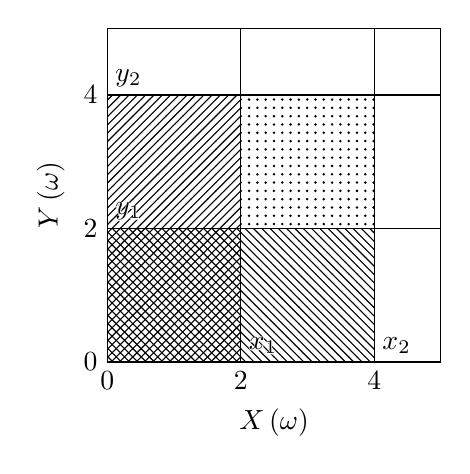
\begin{tikzpicture}
		\begin{axis}[
				xmin=0, xmax=5,
				ymin=0,ymax=5,
				width=0.48\textwidth, height=0.48\textwidth, grid=major, ylabel=$Y\left(\omega \right)$, xlabel=$X\left(\omega \right)$]
			\draw (2,0)--(2,5);
			\draw (4,0)--(4,5);
			\draw (0,2)--(5,2);
			\draw (0,4)--(5,4);
			\draw [pattern = dots](2,2)rectangle(4,4);
			\draw [pattern = north east lines](0,0)rectangle(2,4);
			\draw [pattern = north west lines](0,0)rectangle(4,2);
			\node [anchor = south west, inner sep = 1 , outer sep = 2 pt] at (2,0) {\contour{white}{$ x_1 $}};
			\node [anchor = south west, inner sep = 1 , outer sep = 2 pt] at (4,0) {\contour{white}{$ x_2 $}};
			\node [anchor = south west, inner sep = 1  , outer sep = 2 pt] at (0,2) {\contour{white}{$ y_1 $}};
			\node [anchor = south west, inner sep = 1  , outer sep = 2 pt] at (0,4) {\contour{white}{$ y_2 $}};
		\end{axis}
	\end{tikzpicture}
\end{center}
Nota come le aree costituiscano le diverse probabilità:
\begin{itemize}
	\item \tikz \draw [pattern = dots](0,-0.25)rectangle(0.5,0.25); costituisce  $ \Pr \left(x_1 <  X \le  x_2, y_1 < Y \le  y_2\right) $
	\item \tikz \draw [pattern = north east lines](0,-0.25)rectangle(0.5,0.25); costituisce $ \Pr \left(X \le  x_1,  Y \le  y_2\right)  $
	\item \tikz \draw [pattern = north west lines](0,-0.25)rectangle(0.5,0.25); costituisce $ \Pr \left(X \le  x_2,  Y \le  y_1\right)  $
	\item 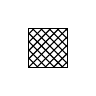
\begin{tikzpicture}
		      \draw [pattern = north west lines](0,-0.25)rectangle(0.5,0.25);
		      \draw [pattern = north east lines](0,-0.25)rectangle(0.5,0.25);
	      \end{tikzpicture} costituisce $ \Pr \left(X \le  x_1,  Y \le  y_1\right)  $
\end{itemize}
quindi dobbiamo togliere dall'area totale i due rettangoli verticali ed orizzontali \tikz \draw [pattern = north east lines](0,-0.25)rectangle(0.5,0.25);,\tikz \draw [pattern = north west lines](0,-0.25)rectangle(0.5,0.25);, e riaggiungere il quadrato piccolo in fondo 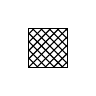
\begin{tikzpicture}
	\draw [pattern = north west lines](0,-0.25)rectangle(0.5,0.25);
	\draw [pattern = north east lines](0,-0.25)rectangle(0.5,0.25);
\end{tikzpicture}, dato che è stato tolto due volte
\vskip3mm
Infine, se è nota la funzione di probabilità congiunta $p_{X, Y}(x, y)$ allora è facile ottenere le funzioni di probabilità delle v.a. $X$ e $Y$
\[
	p_X(X=x)=\sum_{y \in R_Y} p_{X, Y}(x, y) \quad p_Y(Y=y)=\sum_{x \in R_X} p_{X, Y}(x, y)
\]
e quindi
\[
	F_X(x)=\sum_{u \leq x} \sum_{y \in R_Y} p_{X, Y}(u, y) \quad F_Y(y)=\sum_{v \leq y} \sum_{x \in R_X} p_{X, Y}(x, v)
\]
\subsection{V.a. doppie continue}
\definizione{Probabilità di v.a. doppia discreta}{
	La v.a. doppia $Z=(X, Y)$ si dirà dotata di densità se esiste una funzione $f_{X, Y}(x, y)$ tale che
	- $f_{X, Y}(x, y) \geq 0, \forall(x, y) \in \mathbb{R}^2$
	\[
		\int_{-\infty}^{+\infty} \int_{-\infty}^{+\infty} f_{X, Y}(x, y) d x d y=1
	\]
	A questo punto, la probabilità sarà così definita:
	\[
		\Pr(a<x \leq b, c<y \leq d)=\int_a^b \int_c^d f_{X, Y}(x, y) d x d y
	\]
}
Tale funzione è chiamata densità congiunta $f_Z(z)=f_{X, Y}(x, y)$.
Da cui abbiamo
\[
	\begin{gathered}
		F_{X, Y}(x, y)=\int_{-\infty}^x \int_{-\infty}^y f_{X, Y}(u, v) d u d v \\
		f_X(x)=\int_{-\infty}^{+\infty} f_{X, Y}(x, v) d v \quad f_Y(y)=\int_{-\infty}^{+\infty} f_{X, Y}(u, y) d u
	\end{gathered}
\]
Intuitivamente, la probabilità che $ X \in  \left(a,b\right) $ e $ Y \in \left(c,d\right) $ è uguale al volume del "trapezoide" con base $ abcd $ sotteso al grafico della densità di probabilità

\subsubsection*{Esempi funzioni di probabilità doppie}
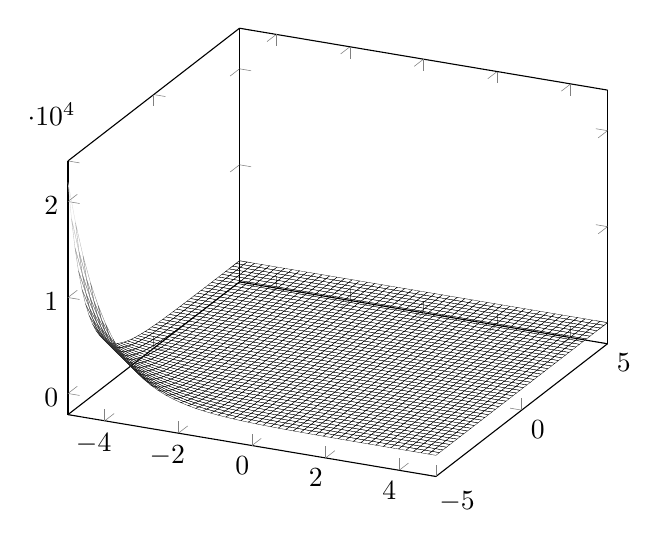
\begin{tikzpicture}
	\begin{axis}[colormap/blackwhite]
		\addplot3[samples = 50, shader=interp, mesh, mesh, ultra thin] {e^(-x-y)};
	\end{axis}
\end{tikzpicture}
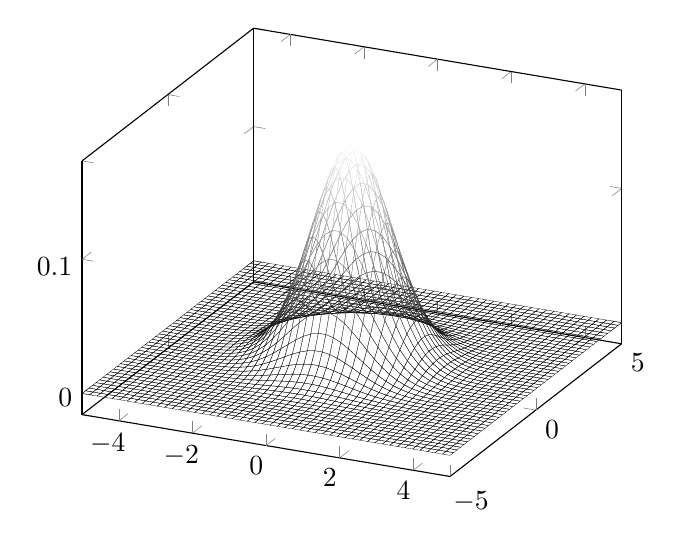
\begin{tikzpicture}
	\begin{axis}[colormap/blackwhite]
		%\addplot3[samples = 50, mesh, draw = black, dotted] {exp(-x^2-y^2-1)};
		\addplot3[samples = 50, shader=interp, mesh, mesh, ultra thin] {1/(2*pi)*exp(-1/2*(x^2+ y^2))};
	\end{axis}
\end{tikzpicture}
\subsection{V.a. condizionata}
\definizione{Distribuzione condizionata di una v.a.}{
	Sia $ \left(\omega , \mathcal{A}, Pr\right) $ uno spazio \underline{probabilizzato}. Sia $ X\left(\omega \right) $ e $ Y\left(\omega \right) $ due v.a. \underline{discrete}. Allora la funzione di probabilità sullo spazio di arrivo è così definita:
	\[
		P_{X | Y} \left(x|y\right) = \frac{P\left(\left\{ X = x\right\} \cap \left\{Y = y\right\}\right)}{P\left(\left\{Y = y\right\}\right)} = \frac{P_{x,y}\left(x,y\right)}{ P_{y} \left(y\right)}
	\]
}
Nota che possiamo definire una v.a. nel modo seguente:
\vskip3mm
Sia $ \left(X, Y\right) \sim P_{x,y} \left(x,y\right) $ \underline{discreta}. Allora
\[
	\forall  y \in  R_y \quad Z_y =  X | y \sim P_{x|y} \left(x | y\right)
\]
ossia $ P_{z_y} \left(x\right) = P\left(X = x | Y = y\right) $. L'idea è quella di \underline{fissare} un valore di $ y $, e costruire una funzione di probabilità che associa ad ogni valore di $ x $ la probabilità di $ x | y $. Chiaramente questa è una v.a. in quanto la somma delle probabilità è 1:
\[
	\sum \frac{P\left(x\right) \cap   P\left(y\right)}{P\left(y\right)} = 1
\]

\subsection{Esempio}
\label{Esempio dado}
Consideriamo le seguenti v.a. che riguardano il lancio di un dado:
\[
	X \left(\omega \right) = \omega  = \text{ numero del dado uscito }
\]
\[
	Y\left(\omega \right) =
	\begin{cases}
		0 & \text{ esce numero dispari }                    \\
		1 & \text{ esce numero pari minore di 4 }           \\
		2 & \text{ esce numero pari maggiore o uguale a 4 }
	\end{cases}
\]
La funzione di probabilità $ p_{x,y} \left(x,y\right) $ associa ad ogni numero coppia ordinata la probabilità dell'insieme intersezione fra $ x $ e $ y $:

\begin{center}
	\begin{table}[H]
		\begin{center}
			\begin{tabular}{|c|ccc|}
				\hline
				            & \multicolumn{3}{c|}{$Y(\omega)$}                                   \\
				$X(\omega)$ & 0                                & 1             & 2               \\
				\hline 1    & $\frac{1}{6}$                    & 0             & 0               \\
				2           & 0                                & $\frac{1}{6}$ & 0               \\
				3           & $\frac{1}{6}$                    & 0             & 0               \\
				4           & 0                                & 0             & $\frac{1}{6}$   \\
				5           & $\frac{1}{6}$                    & 0             & 0               \\
				6           & 0                                & 0             & $ \frac{1}{6} $ \\
				\hline
			\end{tabular}
		\end{center}
		\caption{Funzione di probabilità congiunta}
	\end{table}
\end{center}

\begin{center}
	\begin{table}[H]
		\begin{center}
			\begin{tabular}{|c|ccc|c|}
				\hline
				            & \multicolumn{3}{c|}{$Y(\omega)$} &                                               \\
				$X(\omega)$ & 0                                & 1             & 2             & $F_X(x)$      \\
				\hline 1    & $\frac{1}{6}$                    & $\frac{1}{6}$ & $\frac{1}{6}$ & $\frac{1}{6}$ \\[5pt]
				2           & $\frac{1}{6}$                    & $\frac{2}{6}$ & $\frac{2}{6}$ & $\frac{2}{6}$ \\[5pt]
				3           & $\frac{2}{6}$                    & $\frac{3}{6}$ & $\frac{3}{6}$ & $\frac{3}{6}$ \\[5pt]
				4           & $\frac{2}{6}$                    & $\frac{3}{6}$ & $\frac{4}{6}$ & $\frac{4}{6}$ \\[5pt]
				5           & $\frac{3}{6}$                    & $\frac{4}{6}$ & $\frac{5}{6}$ & $\frac{5}{6}$ \\[5pt]
				6           & $\frac{3}{6}$                    & $\frac{4}{6}$ & 1             & 1             \\[5pt]
				\hline
				$F_Y(y)$    & $\frac{3}{6}$                    & $\frac{4}{6}$ & 1             & /             \\[5pt]
				\hline
			\end{tabular}
		\end{center}
		\caption{Ripartizione probabilità congiunta}
	\end{table}
\end{center}

\begin{center}
	\begin{table}[H]
		\begin{center}
			\begin{tabular}{|c|ccc|}
				\hline
				            & \multicolumn{3}{c|}{$Y(\omega)$}                       \\
				$X(\omega)$ & 0                                & 1 & 2               \\
				\hline 1    & $\frac{1}{3}$                    & 0 & 0               \\
				2           & 0                                & 1 & 0               \\
				3           & $\frac{1}{3}$                    & 0 & 0               \\
				4           & 0                                & 0 & $\frac{1}{2}$   \\
				5           & $\frac{1}{3}$                    & 0 & 0               \\
				6           & 0                                & 0 & $ \frac{1}{2} $ \\
				\hline
			\end{tabular}
		\end{center}
		\caption{Probabilità condizionata}
	\end{table}
\end{center}
In quest'ultimo caso, pensa di fissare un valore di $ Y $, considerando dunque $ Z_y \sim P\left(x | y\right) $ dove $ y $ è fissato. Questa è una v.a. (se sommi in colonna le probabilità otterrai chiaramente $ 1 $ per ogni colonna). Ora posso calcolare la varianza e media delle v.a. $ Z_y $:
\begin{align*}
	\mathbb{E} \left(Z_0\right)         & = 1 \cdot \frac{1}{3} + 2 \cdot 0 + 3 \cdot \frac{1}{3} + 4 \cdot 0 + 5 \cdot \frac{1}{3} + 6 \cdot 0                        & = 3           \\
	\mathbb{E} \left(Z_1\right)         & =   2 \cdot 1                                                                                                                & = 2           \\
	\mathbb{E} \left(Z_2\right)         & =  4 \cdot  \frac{1}{2} + 5  + 6 \cdot  \frac{1}{2}                                                                          & =5            \\
	\operatorname{Var} \left(Z_0\right) & = 1^2 \cdot \frac{1}{3} + 2^2 \cdot 0 + 3^2 \cdot \frac{1}{3} + 4^2 \cdot 0 + 5^2  \cdot  \frac{1}{3} + 6 ^2  \cdot  0 - 3^2 & = \frac{8}{3} \\
	\operatorname{Var} \left(Z_1\right) & = 2^2  \cdot  1 - 2^2                                                                                                        & = 0           \\
	\operatorname{Var} \left(Z_1\right) & = 4^2 \cdot  \frac{1}{2} + 6^2  \cdot \frac{1}{2} - 5^2                                                                      & = 1
\end{align*}
\subsection{Variabile aleatoria definita dalla speranza matematica}
Data una v.a. condizionale, possiamo definire una seconda variabile aleatoria data da:
\[
	Z = \mathbb{E} \left(X | Y = y\right)
\]
\begin{minipage}[c]{0.38\textwidth}
	\begin{tabular}{|c|ccc|}
		\hline
		            & \multicolumn{3}{c|}{$Y(\omega)$}                       \\
		$X(\omega)$ & 0                                & 1 & 2               \\
		\hline 1    & $\frac{1}{3}$                    & 0 & 0               \\
		2           & 0                                & 1 & 0               \\
		3           & $\frac{1}{3}$                    & 0 & 0               \\
		4           & 0                                & 0 & $\frac{1}{2}$   \\
		5           & $\frac{1}{3}$                    & 0 & 0               \\
		6           & 0                                & 0 & $ \frac{1}{2} $ \\
		\hline
	\end{tabular}
\end{minipage}
%
\begin{minipage}[c]{0.60\textwidth}
	Ad esempio, supponendo che l'esperimento aleatorio abbia dato come esito la coppia $ \left(3,0\right) $, allora la variabile aleatoria $ Z $ collegherebbe questo esito alla media della v.a. $ X | Y = 0 $, ossia $ \mathbb{E} \left(X | Y = 0\right) = 3 $. Tale variabile viene anche chiamata $ \mathbb{E} \left(X | Y\right) $
\end{minipage}
\vskip3mm
La media di $ \mathbb{E} \left(X | Y\right) $ gode della seguente proprietà:
\teorema{Tower property}{
	Date due v.a. $ X $ e $ Y $ e la loro funzione di probabilità condizionata, allora:
	\[
		\mathbb{E}\left(\mathbb{E}\left(X|Y\right)\right) = \mathbb{E}\left(X\right)
	\]
	dove $ \mathbb{E}\left(X|Y\right) $ è la v.a. $ \mathbb{E} \left(X | Y = y\right) $
}
\subsubsection*{Dimostrazione}
\begin{align*}
	\mathbb{E}(\mathbb{E}(X \mid Y)) & =\sum_{y \in R_Y}\left[\sum_{x \in R_x} x p_{X \mid Y}(x \mid y)\right] p_Y(y) \\
	                                 & =\sum_{y \in R_Y} \sum_{x \in R_x} x p_{X \mid Y}(x \mid y) p_Y(y)             \\ & =\sum_{y \in R_Y} \sum_{x \in R_x} x p_{X, Y}(x, y) \\ & =\sum_{x \in R_x} x \sum_{y \in R_Y} p_{X, Y}(x, y) \\ & =\sum_{x \in R_x} x p_X(x)=\mathbb{E}(X)
\end{align*}
\teorema{Teorema di composizione della varianza}{
	Date due v.a. $ X $ e $ Y $ e la loro funzione di probabilità condizionata, allora:
	\[
		\operatorname{Var}\left(X\right) = E\left(\operatorname{Var}\left(X|Y\right)\right) + \operatorname{Var} \left(E\left(X|Y\right)\right)
	\]
	dove $ \mathbb{E} \left(X |Y\right)$ è la v.a. $\mathbb{E}\left(X|Y = y\right) $
}\label{Composizione della varianza}
\subsubsection*{Dimosrazione}
Partiamo dalla definizione di varianza:
\[
	Var \left(X\right) = \sum_{x \in \R x} \left(x - \mathbb{E}\left(x\right)\right)^2 p_x\left(x\right)
\]
\begin{align*}
	\operatorname{Var}(X) & =\sum_{x \in R_X}(x-\mathbb{E}(X))^2 p_X(x)                                                                                                                    \\
	                      & =\sum_{x \in R_X}(x-\mathbb{E}(X))^2 \sum_{x \in A_Y} p_{X Y}(x, y)                                                                                            \\
	                      & =\sum_{x \in R_X} \sum_{y \in R_Y}(x-\mathbb{E}(X | Y=y)+\mathbb{E}(X | Y=y) -\mathrm{E}(X))^2 p_{X,Y}(x, y)                                                   \\
	                      & =\sum_{x \in R_X} \sum_{ y \in R_Y}\left(x-\mathbb{E}(X | Y=y)^2 p_{X, Y}(x, y)\right.                                                                         \\
	                      & +\sum_{x \in R_X} \sum_{y \in R_Y}\left(\mathbb{E}(X) Y=y)-\mathbb{E}(X)\right)^2 p_{X,Y} (x, y)                                                               \\
	                      & +2 \sum_{x \in R_X} \sum_{y \in R_Y}\left(x-\mathbb{E}(X | Y=y)\right)(\mathbb{E}(X | Y=y)-E(X))p_{X,Y} \left(x,y\right)                                       \\
	                      & =\sum_{y \in  R_Y}\left[\sum_{x \in R_X}\left(x-\mathbb{E}\left(X | Y=y\right)^2 p_{X| Y}(x | y)\right)\right] p_Y(y)                                          \\
	                      & +\sum_{y \in R_Y}\left[\sum_{x \in  R_X}\left(\mathbb{E}(X | Y=y)-\mathbb{E} \left(\mathbb{E}\left(X | Y\right)\right)\right)^2 p_{X | Y}(x | y)\right] p_Y(y) \\
	                      & +0                                                                                                                                                             \\
	                      & =\mathbb{E}(\operatorname{Var}(X | Y))+\operatorname{Var}(\mathbb{E}(X | Y))                                                                                   \\
	                      &
\end{align*}

Rimane da mostrare

\[
	2 \sum_{x \in R_X} \sum_{y \in R_Y}(x-\mathbb{E}(X | Y=y))(\mathbb{E}\{X | Y=y)-\mathbb{E}\{X)\} p_{X, Y}(x, y)=0
\]
infatti
\begin{align*}
	 & =\sum_{ x \in R_X} \sum_{y \in R_Y}(x-\mathbb{E}(X | Y=y)\rangle(\mathbb{E}(X | Y=v)-\mathbb{E}(X))p_{X, Y}\left(x, y\right)                             \\
	 & =\sum_{y \in R_Y}\left(\mathbb{E}(X | Y=y) -\mathbb{E}(X)\right)\left[\sum_{x \in R_X}(x-\mathbb{E}(X | Y=y)) p _{ X | Y}(x | y)\right] p_Y(y)           \\
	 & =\sum_{y \in R_Y}\left(\mathbb{E}(X | Y=y) -\mathbb{E}(X)\right)\left[\sum_{x \in R_X}x  p_{X | Y}\left(x|y\right) - \mathbb{E}(X | Y=y)) \right] p_Y(y) \\
	 & =\sum_{y \in R_y}(\mathbb{E}(X | Y=y)-\mathbb{E}(X))\left[\mathbb{E}(X | Y=y)-\mathbb{E}(X | Y=y)\right]  p_Y(y)                                         \\
\end{align*}
\subsubsection*{Applicazione teorema}
Ritornando all'esericio in sub \ref{Esempio dado}
\begin{align*}
	\mathbb{E}(\operatorname{Var}(X \mid Y)) & =\left[\frac{8}{3} \cdot  \frac{1}{2}+ 0 \cdot \frac{1}{6}+1 \cdot \frac{1}{3}\right]=\frac{8}{6}+\frac{2}{6}=\frac{10}{6}                     \\
	\operatorname{Var}(\mathrm{E}(X \mid Y)) & = \left[3^2  \cdot \frac{1}{2} + 2^2  \cdot \frac{1}{6} + 5^2  \cdot \frac{1}{3}\right] - \mathbb{E} \left(\mathbb{E}\left(X|Y\right)\right)^2 \\
	                                         & = \left[\frac{81}{6}\right] - \mathbb{E} \left(X\right)^2  = \frac{27}{2} - \frac{49}{4} = \frac{5}{4}                                         \\
	\operatorname{Var}(X)                    & =\left[(1-3.5)^2+(2-3.5)^2+(3-3.5)^2+(4-3.5)^2\right]\frac{1}{6} = \frac{35}{12}                                                               \\
\end{align*}

Se non avessimo conosciuto la distribuzione di $ X $, avremmo potuto utilizzare il teorema \ref{Composizione della varianza}:
\[
	\operatorname{Var} \left(X\right) = \frac{11}{6} + \frac{5}{4}  = \frac{35}{12}
\]
\subsection{Misure di dipendenza fra v.a.}
Si possono definire degli indici per quantificare quanto e come una variabile aleatoria $ X $ influenzi il risultato di una variabile aleatoria $ Y $
\definizione{Indipendenza stocastica fra v.a.}{
	$ \left(X, Y\right) $ sono \underline{stocasticamente indipendenti} se
	\[
		P_{X, Y} \left(x,y\right) = P_{X }\left(x\right) P_{Y}\left(y\right) \quad  \forall \left(x,y\right) \in  R_X \times R_Y
	\]
}

Nota che se due variabili sono stocasticamente indipendenti vale che:
\[
	P\left(X|Y\right) = \frac{P_{X,Y}\left(x,y\right)}{P\left(y\right)} = \frac{P_X\left(x\right) \cdot  P_Y\left(y\right)}{P_Y\left(y\right)} = P_X\left(x\right)
\]
\definizione{Indipendenza in media}{
	Date $ \left(X,Y\right) $ si dice che $ X $ è \underline{indipendente in media} da $ Y $ se :
	\[
		\mathbb{E}\left(X|Y=y\right) = \mathbb{E} \left(X\right) \forall y \in  R_Y
	\]
}
Mentre l'indipendenza stocastica indica che un evento $ y $ non influenza in alcun modo un evento $ x $, l'indipendenza in media indica che un evento $ y $ non influenza la media nel verificarsi di $ x $ dato $ y $
\vskip3mm
Nota bene che:
\begin{itemize}
	\item A differenza dell'indipendenza stocastica, \underline{l'indipendenza in media non è simmetrica}: il fatto che $ X $ sia indipendente in media da $ Y $ non implica che $ Y $ sia indipendente in media da $ X $
	\item Se due v.a. sono stocasticamente indipendenti, allora lo sono anche in media
\end{itemize}
Inoltre è possibile quantificare quanto la media di una variabile $ X $ sia influenzata da quella di un'altra $ Y $ tramite l'\textit{indice di dipendenza in media}
\definizione{Rapporto di correlazione}{
Sia $ \left(X, Y\right) $ una v.a. doppia discreta, si chiama rapporto di correlazione di $ X $ dato $ Y $
\[
	n^2 _{X|Y} = \frac{\operatorname{Var} \left(\mathbb{E}\left(X|Y\right)\right)}{\operatorname{Var}\left(X\right)} = 1 - \frac{\mathbb{E}\left(\operatorname{Var} \left(\mathbb{E}\left(X|Y\right)\right)\right)}{\operatorname{Var}\left(X\right)} \quad  \operatorname{Var} \left(X\right) > 0
\]
in modo analogo si definisce $ n^{2}_{Y|X} $
}
Dalla formula della scomposizione della varianza è facile vedere che
\[
	0 \leq \eta_{X \mid Y}^2 \leq 1
\]
inoltre
\begin{itemize}
	\item se $\eta_{X \mid Y}^2=0$ allora $X$ è indipendente in media da $Y$;
	\item se $\eta_{X \mid Y}^2>0$ allora $X$ è dipendente in media da $Y$;
	\item $\eta_{X \mid Y}^2=1$ se e solo se $\Pr(X=\mathbb{E}(X \mid Y))=1$.
\end{itemize}
\definizione{Covarianza e correlazione}{
	La covarianza e la correlazione sono altri due indici di dipendenza (lineare) tra due v.a..
	\[
		\mathbb{C}ov(X, Y)=\mathbb{E}(X \cdot Y)-\mathbb{E}(X) \cdot \mathbb{E}(Y)
	\]
	mentre
	\[
		\rho(X, Y)=\frac{\mathbb{C}ov(X, Y)}{\sqrt{\mathbb{V}ar(X) \cdot \mathbb{V} a r(Y)}}
	\]
}
\teorema{Varianza di una combinazione lineare di v.a.}{
	Sia $(X, Y)$ una v.a. doppia e $ a $ e $ b $ due costanti. Allora
	\[
		\mathbb{V} a r(a X+b Y)=a^2 \mathbb{V} a r(X)+b^2 \mathbb{V} a r(Y)+2 a b \mathbb{C} o v(X, Y)
	\]
}
\section{Teoremi limite della probabilità}
\subsection{La legge dei grandi numeri}
Immaginiamo di lanciare un dado $ n $ volte. Intuitivamente avremo che il numero di volte che è uscito il numero $ 3 $, fratto il numero di lanci, per $ n $ "molto grande", convergerà alla probabilità che esca $ 3 $. Questo è proprio il ragionamento intuitivo alla base della legge dei grandi numeri
\definizione{Convergenza in probabilità (o debole)}{
	Sia $ S $ una v.a. binomiale (che conta il numero di successi in $ n $ tentativi). Sia $ p $ la probabilità del successo. Allora si dice che per $ n \to  \infty  $ la v.a. \underline{converge in probabilità}, ossia accade che per $ \varepsilon $ piccolo a piacere:
	\[
		\lim_{n \to \infty} \Pr\left\{\left|\frac{S_n}{n} - p\right| \ge \epsilon \right\} = 0
	\]
	In simboli si scrive che $ \frac{S_n}{n} \xrightarrow{p} p   $
}
Si può dire equivalentemente che $ Z_i \xrightarrow{p}Z  $ se:
\[
	\lim_{i \to \infty} Pr\left( \left|Z_i - Z\right| > \epsilon \right) = 0
\]
per ogni $ \epsilon  $ piccolo a piacere
\vskip3mm
Allo stesso modo, se fossimo interessati agli scotamenti al quadrato, potremmo ricorrere al concetto di convergenza in media quadratica
\definizione{Convergenza in media quadratica}{
	Sia $ S $ una v.a. binomiale (che conta il numero di successi in $ n $ tentativi). Sia $ p $ la probabilità del successo. Allora si dice che per $ n \to  \infty  $ la v.a. \underline{converge in media}, ossia accade che per $ \varepsilon $ piccolo a piacere:
	\[
		\lim_{n \to \infty} \mathbb{E}\left[\left(\frac{S_n}{n} - p\right)^2 \right] = 0
	\]
	In simboli si scrive che $ \frac{S_n}{n} \xrightarrow{m.q.} p   $
}
Anche in questo caso si può scrivere che $ Z _i \xrightarrow{m.q} Z $ se
\[
	\lim_{n \to \infty } \mathbb{E} \left[\left(Z_n - Z\right)^2 \right] = 0
\]
\teorema{Convergenza in media e in probabilità}{
	La convergenza in media quadratica implica la convergenza in probabilità, ma non viceversa:
	\[
		Y_n \xrightarrow{m.q.} Y \Rightarrow Y_n \xrightarrow{P} Y
	\]
}
\subsubsection*{Somma variabili aleatorie e teoremi utili in statistica}

\teorema{Media e varianza della maedia campionaria}{
	Siano $Y_1, \ldots, Y_n$ v.c. indipendenti, tutte con valore atteso $\mu$ e varianza $\sigma^2$ e sia $\bar{Y}_n=\sum_{i=1}^n Y_i / n$. Allora
	\begin{align*}
		\mathbb{E}\left(\bar{Y}_n\right)         & =\sum_{i=1}^n \frac{\mathbb{E}\left(Y_i\right)}{n}=n \frac{\mu}{n}=\mu,                              \\
		\operatorname{Var}\left(\bar{Y}_n\right) & =\sum_{i=1}^n \frac{\mathbb{V} a r\left(Y_i\right)}{n^2}=n \frac{\sigma^2}{n^2}=\frac{\sigma^2}{n} .
	\end{align*}
}
\teorema{Legge debole dei grandi numeri }{
	Sia $Y_1, Y_2, \ldots$ una successione di v.c. indipendenti, ciascuna con valore atteso $\mu$ e varianza $\sigma^2$. Sia $\bar{Y}_n=\sum_{i=1}^n Y_i / n$, allora, per ogni $\varepsilon>0$,
	\[
		\lim _{n \rightarrow \infty} \Pr\left\{\left|\bar{Y}_n-\mu\right| \geq \varepsilon\right\}=0,
	\]
	ovvero $\bar{Y}_n \stackrel{P}{\longrightarrow} \mu$.
}
Questo esprime il seguente concetto intuitivo: se ripetiamo $ n $ volte un esperimento che ha probabilità $ p $ di dare successo, allora la media campionaria tenderà a $ p $ per $ n $ molto grande, ossia:
\[
	\frac{\text{numero successi}}{\text{numero tentativi}} \to p \quad \text{ per } n \text{ molto grande }
\]
\subsubsection*{Dimostrazione}
\[
	\mathbb{E} \left[\left(Y - \mu \right)^2 \right] = \operatorname{Var}\left(\overline{Y}_n\right) = \frac{\sigma ^2 }{n}  \to  0
\]
\subsubsection*{Teorema del limite centrale}
\teorema{Teorema del limite centrale}{
	Sia $Y_1, Y_2, \ldots$ una successione di v.c. ciascuna con $\mathbb{E}\left(Y_i\right)=\mu $ e $ \mathbb{V} a r\left(Y_i\right)=\sigma^2$. Allora, posto $Z_n=$ $\sqrt{n}\left(\bar{Y}_n-\mu\right) / \sigma$, per ogni $z$
	\[
		\lim _{n \rightarrow \infty} \operatorname{Pr}\left(Z_n \leq z\right)=\frac{1}{\sqrt{2 \pi}} \int_{-\infty}^z e^{-t^2 / 2} d t .
	\]
	In simboli il teorema del limite centrale si denota scrivendo
	\[
		Z_n=\sqrt{n} \frac{\left(\bar{Y}_n-\mu\right)}{\sigma} \stackrel{\mathcal{D}}{\longrightarrow} \mathcal{N}(0,1),
	\]
	dove $\stackrel{\mathcal{D}}{\longrightarrow}$ si legge "converge in distribuzione".
	Una lettura grezza (ma pratica) del teorema del limite centrale è la seguente:
	\[
		\bar{Y}_n \stackrel{a}{\sim} \mathcal{N}\left(\mu, \frac{\sigma^2}{n}\right)
	\]
	dove $\stackrel{a}{\sim}$ significa "distribuita approssimatamente".
}
In poche parole, si intende che per valori di $ n $ molto grandi, una v.a. che rappresenta la \underline{media} di una distribuzione binomiale può essere approssimata con una distribuzione \underline{normale di parametri} $ \mu  $ e $ \frac{\sigma ^2 }{n} $
\subsubsection*{Approssimazione binomiale con v.a. normale}
Se sono verificare le seguenti condizioni posso approssimare una v.a. binomiale con una normale:
\begin{itemize}
	\item $ n $ è abbastanza grande
	\item $ p $ e $ 1-p $ sono piuttosto lontani da 0
	\item L'intervallo $ \left[np \pm \sqrt{np\left(1-p\right)}\right] $ è contenuto nell'intervallo $ \left[0,n\right] $
\end{itemize}
\teorema{Approssimazione della binomiale con una normale}{
	Una v.a. $ X \sim \mathcal{B}\left(n,p\right) $ si può approssimare con una v.a. normale con parametri di valore :
	\[
		\mu  = np \quad  \sigma ^2  = np\left(1-p\right)
	\]
	Nel calolo del valore standardizzato devo aggiungere la cosiddetta \underline{correzione per continuità} = $ 0.5 $, che migliora la precisione dell'approssimazione
}
Ad esempio data $ X \sim \mathcal{B}\left(n, p\right) $, se dovessi calcolare $ \Pr \left(X < 25\right) $ allora il valore standardizzato di 25 è
\[
	\frac{\left(25 + \textbf{0.5}\right) - \mu }{ \sigma } =  \frac{\left(25 + \textbf{0.5}\right) - np}{\sqrt{np\left(1-p\right)}}
\]
\subsubsection*{Diseguaglianze utili}
\teorema{Disuguaglianza di Markov}{
	Sia $ Y $ una v.a. che assume valori \underline{non negativi}, allora per ogni numero reale $ a > 0 $ si ha che :
	\[
		\Pr \left(Y \ge  a\right) \le  \frac{\mathbb{E}\left(Y\right)}{a}
	\]
}
\teorema{Disuguaglianza di Chebychev}{
	Sia $ Y $ una v.a. con valore atteso $ \mathbb{E}\left(Y\right) = \mu  $ e varianza $ Var \left(Y\right) = \sigma ^2  $, allora:
	\[
		\Pr \left(\left|Y - \mu \right| \ge  \epsilon \right) \le  \frac{\sigma  ^2 }{ \mu^2 }
	\]
}
Tali disuguaglianze sono molto utili in quanto ci permettono di conoscere "i limiti" di una v.a., senza tuttavia conoscerne la sua distribuzione.
\subsubsection*{Esempio utilizzo diseguaglianze}
Supponiamo che una v.a. $ X $ conti il numero di auto prodotte in una settimana da una fabbrica. Sappiamo che in media ne vengono prodotte 50, ossia $ \mathbb{E}\left(X\right) = 50 $. Allora possiamo affermare che
\begin{itemize}
	\item $\Pr\left(X > 75\right) \le \frac{50}{75} = \frac{2}{3} $ per \underline{disuguaglianza di Markov}
	\item Supponendo che la varianza sia $ 25 $, cosa posso dire circa la probabilità che vengano prodotte fra le 40 e le 60 auto? Procedo con la disuguaglianza di Chebychev
	      \begin{align*}
		      \Pr \left(40 < Y < 60 \right) & = \Pr \left(-10, Y- 50 < 10\right)             \\
		                                    & = \Pr\left(\left|Y-50\right| < 10\right)       \\
		                                    & = 1 -\Pr\left(\left|Y- 50\right| \ge 10\right)
	      \end{align*}
	      sapendo che per la \underline{disuguaglianza di Chebychev}
	      \[
		      \Pr\left(\left| Y - 50\right| \ge  10\right)\le \frac{Var \left(Y\right)}{\mathbb{E} \left(X\right)^2 } = \frac{25}{100} = \frac{1}{4}
	      \]
	      avrò che
	      \[
		      \Pr\left(40 < Y < 60\right) = 1 -\Pr\left(\left|Y - 50\right| \ge  10\right) \ge \frac{3}{4}
	      \]
\end{itemize}
\section{Inferenza statistica}
Tramite l'inferenza statistica, vogliamo utilizzare dei dati raccolti per poter creare modelli probabilistici e dare affermazioni su di una data popolazione
\subsubsection*{Popolazione, campione, unità statistiica}
\begin{center}
	\begin{tikzpicture}
		%\draw (0,0)ellipse(2 and 1);
		\node (camp)[circle, draw, inner sep = 20] at (0,0) {};
		\node (pop)[ellipse, draw,inner xsep = 50 ,inner ysep = 30] at (0,0) {};
		\node [] at (0,0) {x};
		\node [] at (0.4,0.2) {x};
		\node [] at (-0.4,0.2) {x};
		\node (ind)[] at (-0.2,-0.4) {x};
		\node [] at (0.4,-1.2) {x};
		\node [] at (-0.9,-1.15) {x};
		\node [] at (2,0) {x};
		\node [] at (1.6,0.3) {x};
		\node [] at (1.8,-0.3) {x};
		\node [] at (-1.8,-0.3) {x};
		\node [] at (-2,0.3) {x};
		\node [anchor = east] at (-3, -2) {Campione};
		\draw (-3, -2)--(camp);
		\node [anchor = west] at (3, -2) {Popolazione di riferimento};
		\draw (3, -2)--(pop);
		\node [anchor = north] at (0, -2) {Unità statistica};
		\draw (ind)--(0,-2);
	\end{tikzpicture}
\end{center}
\subsection{Stima e stimatore e metodo dei momenti}
\definizione{Stima}{
	Definiamo \underline{stima} di un parametro un \underline{valore numerico} che può essere ottenuto dai dati raccolti
}
\definizione{Stimatore}{
	Uno stimatore è una qualsiasi \underline{funzione} che prenda in input i dati di un campione e stimi il valore di un determinato parametro.
	\vskip3mm
	Uno stimatore può essere visto anche come una v.a. funzione delle variabili aleatorie che generano i valori osservati nel campione.
	\vskip3mm
	Uno stimatore di un parametro $ \theta $ viene indicato con $ \hat{\theta} $. Talvola $ \hat{\theta } $ indica anche \underline{la stima} del parametro
}
Ad esempio, suppongo di aver una fabbrica che produce lastre di metallo e ottengo i seguenti valori:
\begin{center}
	\begin{tabular}{|ccccc|}
		\hline
		14.33 & 14.19 & 14.39 & 14.43 & 14.17 \\
		\hline
	\end{tabular}
\end{center}
in questo caso posso creare uno stimatore della media con il metodo che viene sempre comunemente utilizzato:
\[
	\hat{\mu } = \frac{1}{n} \sum_{i=1}^{5} x_i
\]
dove $ x_1, \ldots x_5 $ sono le v.a. che indicano lo spessore dell'i-esima lastra
\subsubsection*{Proprietà stimatori}
Idealmente, uno stimatore dovrebbe essere uguale al valore del parametro teorico (ad esempio $ \hat{\mu } = \mu  $). Tuttavia questo non ha senso in quanto implicherebbe di conoscere con certezza il parametro da stimare. Un requisito più ragionevole è la \underline{non distorsione}
\definizione{Non distorsione di uno stimatore}{
	Uno stimatore $ \hat{\theta } $ si dice \underline{non distorto} se
	\[
		\mathbb{E}\left[\left(\hat{ \theta } - \theta \right)\right] = \mathbb{E} \left(\hat{\theta }\right) - \theta = 0
	\]
	ossia gli errori in media di compensano, o meglio, le imprecisioni di distribuiscono in \underline{manira simmetrica} attorno al valore teorico
}
se invece siamo interessati a capire di quanto erra in media uno stimatore possiamo ricorrere al concetto di \underline{errore quadratico medio}
\definizione{Errore quadratico medio di uno stimatore}{
	L'\underline{errore quadratico medio} di uno stimatore $ \hat{\theta } $ è così definito:
	\[
		EQM\left(\hat{\theta }\right) = \mathbb{E}\left[\left(\hat{ \theta } - \theta  \right)^2 \right]
	\]
	Dati due simatori è da preferire in genere quello con l'errore quadratico medio \underline{minore}
}
Nota che:
\[
	EQM\left(\hat{\theta }\right) = \underbracket[0.1ex]{\Var \left(\hat{ \theta }\right)}_{\text{ varianza }} + \underbracket[0.1ex]{\left(\mathbb{E}\left(\hat{\theta }  \right)- \theta\right)^2}_{\text{ distorsione }}
\]
\subsubsection*{Consistenza stimatori}
\definizione{Consistenza stimatorii}{
	Uno stimatore si dice \underline{consistente media quadratica} se
	\[
		EQM \left(\hat{\theta }\right) \to 0
	\]
	mentre si dice \underline{consistente in senso debole} se
	\[
		\hat{ \theta } \xrightarrow{P}  \theta
	\]
}
Nota che ha senso parlare di convergenza in quanto ogni osservazione (ad esempio ogni misura di una lastra di metallo), corrisponde ad una v.a. Dunque uno stimatore sarà dato da una funzione di $ n $ v.a.
\subsubsection*{Metodo dei momenti}
Un modo per "creare" degli stimatori è secondo il metodo dei momenti. Innanzitutto diamo la definizione di momento campionario:
\definizione{Momento campionario}{
Il momento campionario di ordine $ r $ è così definito:
\[
	\mu _r = \frac{1}{n}\sum_{i=1}^{n} X_i^{r}
\]
se dovessi calcolare il momento capionario di una trasformazione $ g\left(X\right) $ di v.a. (ad esempio il momento centrato), allora vale che
\[
	\mu _r = \frac{1}{n} \sum_{i=1}^{n} g\left(X_i\right)^{r}
\]
}
Il metodo dei momenti consiste nel eguagliare l'espressione di un momento teorico con il suo corrispondente momento campionario, ad esempio, supponendo di avere $ X \sim \mathcal{N}\left(\mu , \sigma ^2 \right) $, allora
\begin{align*}
	\mu       & = \mathbb{E} \left(X\right) = \frac{1}{n} \sum_{i = 1}^{n} X_{i}                                            \\
	\sigma ^2 & = \mathbb{E} \left[\left(X - \mu \right)^2  \right]  = \frac{1}{n} \sum_{i=1}^{n} \left(X_i - \mu \right)^2
\end{align*}
\subsection{Metodo della massima verosimiglianza}
Supponiamo di avere un set di campioni derivati dal lancio di una moneta:
\begin{center}
	\begin{tabular}{|cccccccccc|}
		\hline
		$T$ & $ T$ & $C $ & $C $ & $T $ & $T $ & $T $ & $ T$ & $ C$ & $ C$ \\
		\hline
	\end{tabular}
\end{center}
Voglio stimare il parametro $ p $, ossia la probabilità che esca $ T $. Allora
\textbox{Il metodo della massima verosimiglianza ricerca il valore di $ p $ tale per cui la \underline{probabilità} che escano i dati del campione \underline{sia massima}}
La \underline{verosimiglianza} è quindi così definita: 
\[
  L\left(\theta \right) = \Pr \left(\left\{T,T,C,C,T,C,T,T,C,C\right\}\right) = p^{6} \left(1-p\right)^{4}
\]
\begin{itemize}
  \item La verosimiglianza è dunque una funzione di $ p $ ossia del parametro che vogliamo stimare. Per ottenere una legge di distribuzione quanto più accurata possibile devo cercare di massimizzare la probabilità che si verifichi una formazione come quella del campione ($ \left\{T,T,C,C,T,T,T,T,C,C\right\} $)
  \item La \underline{massima verosimiglianza} (o \underline{MLE}) è il valore di $ p $ che rende massima la verosimiglianza
  \item Visto che per trovare il massimo bisogna derivare un prodotto e questo può essere molto tedioso, spesso si utilizza la \underline{log-likelihood}, ossia si applica il logaritmo alla massima verosimiglianza (il log è crescente e non altera i massimi), in modo da trasformare i prodotti in somme
\end{itemize}
\subsubsection*{Valori noti di MLE}
\begin{itemize}
  \item \underline{Normale} 
    \[
          \hat{\mu } = \overline{X}_n  \quad \quad \hat{\sigma ^2 } = \frac{1}{n-1} \sum_{i=1}^{n} \left(X_i - \overline{X_n}\right)^2 
    \]
    \textit{I valori sono distribuiti uniformemente intorno alla media $ \mu  $, per questo la media campionaria approssima bene la media teoria. La varianza è data dalla media di quanto u valore si discosta dalla media}
    \item \underline{Esponenziale}
      \[
      \hat{\lambda } = \frac{1}{\overline{X}_n}
      \]
      \textit{$ \lambda $ è inversamente proporzionale alla media delle osservazioni, più la media è vicina a zero, più lambda sarà alto}
    \item \underline{Bernoulli}
      \[
       \hat{p} = \overline{X} _n = \frac{1}{n} \sum_{i=1}^{n} X_i
      \]
      \textit{Immagina il lancio ripetuto di una moneta per convincertene. E' chiaro che la miglior approssimazione di $ \mu  $ è data dal rapporto fra successi e insuccessi}
    \item \underline{Poisson}
      \[
      \hat{\sigma }  = \overline{X} _n = \frac{1}{n} \sum_{i=1}^{n} X_i
      \]
      \item \underline{Uniforme}, che ha quindi densità
         
        \[
        X_i \sim f = \begin{cases}
          \frac{1}{\sigma } & \text{ se } x \in \left[0, \sigma \right]\\ 
          0 & \text{ altrove }
        \end{cases}
        \]
         allora 
         \[
           \hat{\sigma } = \operatorname{max} \left\{X_1, X_2,\ldots ,X_n\right\}
         \]
         \textit{Se ci pensi ciò significa che i dati si distribuiscono in maniera uniforme nel range $ \left[0, \sigma \right] $ e non ce ne possono essere maggiori di $ \sigma  $ stesso. La stima migliore è il dato più alto registrato}
\end{itemize}
\subsection{Errore di stima ed intervalli di confidenza}
\definizione{Errore di stima}{
  Dato un parametro $ \theta  $, si definisce errore di stima la seguente quantità: 
  \[
  \hat{\theta } - \theta 
  \]
}
Si può calcolare la probabilità che un errore di stima sia "piccolo", ossia \underline{minore della varianza}. Ciò significa prendere la v.a. $ \hat{\theta } - \theta   \sim  \mathcal{N} \left(0, \frac{\sigma ^2}{n} \right)$ e calcolare la probabilità dell'intervallo $ \left[\overline{X}_n- \Var , \overline{X}_n+ \Var \right] $
\definizione{Intervallo di confidenza}{
  Un intervallo è detto \underline{intervallo di confidenza} di livello $ \alpha \in \left(0,1\right) $  se la probabilità che la stima di un parametro ignoto rientri all'interno di esso è $ \alpha  $
}
Per ragioni di comodità di calcolo, spesso l'intervallo di confidenza si indica con $ 1-\alpha  $
\vskip3mm
Praticamente questo servirà quando si andrà a calcolare intorno alla media di una normale l'intervallo di livello $ \alpha  $, ossia l'intervallo tale che 
\[
\Pr \left(x \in \left[\mu + x , \mu -x\right]\right)=\alpha 
\]
\begin{center}
  \begin{tikzpicture}
  \begin{axis}[
      xmin=-4, xmax=4,
      ymin=0,ymax=0.5,
      restrict y to domain = 0:0.5, domain=-4:4, width=0.48\textwidth, height=0.48\textwidth, grid=major, samples=200,  ylabel=$f(x)$, xlabel=$x$, legend entries={{}{$N\left(0,1\right)$}}]
    \def\myomega{1}
    \def\mymu{0}
    \addplot[pattern = north east lines ,draw =none, domain = -2:2] {1/(sqrt(2*pi*\myomega^2))*e^(-1/2*((x-\mymu)^2)/(\myomega^2))}\closedcycle;
    \addplot[black, thick] {1/(sqrt(2*pi*\myomega^2))*e^(-1/2*((x-\mymu)^2)/(\myomega^2))};
    \node (sx)[blackdot] at (-2, {1/(sqrt(2*pi*\myomega^2))*e^(-1/2*(((-2)-\mymu)^2)/(\myomega^2))}) {};
    \node (dx)[blackdot] at (2, {1/(sqrt(2*pi*\myomega^2))*e^(-1/2*((2-\mymu)^2)/(\myomega^2))}) {};
    \draw [dashed] (-2,0)--(sx);
    \draw [dashed] (2,0)--(dx);
  \end{axis}
\end{tikzpicture} 
\end{center}
L'area del trapezoide \tikz[scale = 0.5] \draw [pattern = north east lines](0,0)rectangle(1,1); è uguale ad $ \alpha  $, supponendo che l'intervallo $ -2,2 $ sia di livello $ \alpha  $
\end{document}
